\documentclass[12pt,a4paper]{article}

%% ---------- mathematics ----------
\usepackage{amsmath,amsthm,amssymb,mathtools}

%% ---------- graphics & diagrams ----------
\usepackage{tikz}
\usetikzlibrary{arrows.meta,positioning,shapes.geometric,calc,fit,backgrounds,matrix,decorations.pathreplacing}
\usepackage{graphicx}

%% ---------- tables ----------
\usepackage{booktabs,tabularx,multirow,longtable,array}

%% ---------- algorithms ----------
\usepackage[ruled,vlined,linesnumbered]{algorithm2e}

%% ---------- coloured boxes ----------
\usepackage[most]{tcolorbox}

%% ---------- hyperlinks & cross-refs ----------
\usepackage{hyperref}
\usepackage[capitalize,noabbrev]{cleveref}

%% ---------- page layout ----------
\usepackage[margin=1in]{geometry}
\usepackage{fancyhdr}
\usepackage{enumitem}
\usepackage{xcolor}

%% ---------- fonts & misc ----------
\usepackage{microtype}

%% ============================================================
%%  Custom tcolorbox environments
%% ============================================================
\newtcolorbox{keyinsight}[1][]{%
  colback=blue!5!white,colframe=blue!75!black,
  fonttitle=\bfseries,title=Key Insight,#1}

\newtcolorbox{example}[1][]{%
  colback=green!5!white,colframe=green!75!black,
  fonttitle=\bfseries,title=Example,#1}

\newtcolorbox{warningbox}[1][]{%
  colback=red!5!white,colframe=red!75!black,
  fonttitle=\bfseries,title=Warning,#1}

%% ============================================================
%%  amsthm environments
%% ============================================================
\newtheorem{theorem}{Theorem}[section]
\newtheorem{lemma}[theorem]{Lemma}
\newtheorem{definition}{Definition}[section]
\newtheorem{remark}{Remark}[section]
\newtheorem{proposition}[theorem]{Proposition}
\newtheorem{corollary}[theorem]{Corollary}

%% ============================================================
%%  Custom commands (collected from all sessions in this file)
%% ============================================================
\newcommand{\vect}[1]{\mathbf{#1}}
\newcommand{\sgn}{\operatorname{sgn}}
\newcommand{\step}{\operatorname{step}}
\newcommand{\R}{\mathbb{R}}

\pagestyle{fancy}
\fancyhf{}
\lhead{\textsc{Deep Learning} --- IIIT Dharwad}
\rhead{Perceptron, Linear Separability, and MLP Motivation}
\rfoot{Page \thepage}
\lfoot{Prof.\ S R M Prasanna \& Dr.\ Sunil Saumya}
\renewcommand{\headrulewidth}{0.4pt}

\title{%
  {\Large\bfseries Deep Learning Course}\\[6pt]
  {\LARGE Perceptron, Linear Separability, and MLP Motivation}\\[4pt]
  {\normalsize IIIT Dharwad --- M.Tech Programme}
}
\author{Prof.\ S R M Prasanna \& Dr.\ Sunil Saumya}
\date{Sessions 3, 4}

\begin{document}

\maketitle
\tableofcontents
\clearpage

%% ============================================================
%% Session 03: The Perceptron
%% ============================================================
\part{Session 03: The Perceptron}

%=============================================================

%-------------------------------------------------------------
% Title Page
%-------------------------------------------------------------
\begin{titlepage}
  \centering
  \vspace*{2cm}

  {\Huge\bfseries Deep Learning\par}
  \vspace{0.4cm}
  {\Large\bfseries Session 03 Lecture Notes\par}
  \vspace{1.2cm}

  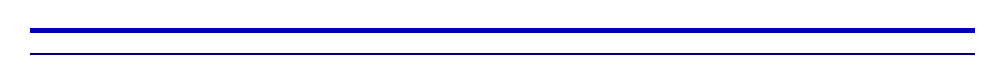
\begin{tikzpicture}
    \draw[blue!70!black, line width=2pt] (0,0) -- (12,0);
    \draw[blue!40!black, line width=0.8pt] (0,-0.3) -- (12,-0.3);
  \end{tikzpicture}

  \vspace{1.0cm}
  {\LARGE\bfseries The Perceptron:\par}
  \vspace{0.3cm}
  {\large From Biological Neurons to Multilayer Networks\par}
  \vspace{1.5cm}

  \begin{tabular}{ll}
    \textbf{Topic:}       & Biological Neurons $\to$ McCulloch-Pitts Model $\to$
                            Perceptron $\to$ MLP \\[4pt]
    \textbf{Session:}     & 03 \\[4pt]
    \textbf{Duration:}    & 1 hour 26 minutes 48 seconds \\[4pt]
    \textbf{Instructors:} & Prof.\ S~R~M~Prasanna \& Dr.\ Sunil Saumya \\[4pt]
    \textbf{Institute:}   & IIIT Dharwad \\[4pt]
    \textbf{Slide Decks:} & \texttt{02-DL-NNIntro} (slides 13--18)
                            \& \texttt{03-DL-Perceptron} (slides 5--14) \\[4pt]
    \textbf{Video:}       & \url{https://vimeo.com/1140267865} \\
  \end{tabular}

  \vspace{2cm}

  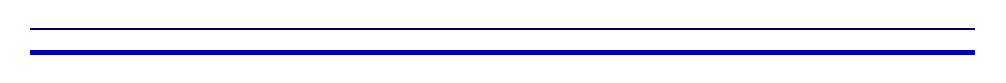
\begin{tikzpicture}
    \draw[blue!70!black, line width=2pt] (0,0) -- (12,0);
    \draw[blue!40!black, line width=0.8pt] (0,0.3) -- (12,0.3);
  \end{tikzpicture}

  \vfill
  {\small These notes synthesise the lecture transcript and visual extractions.
  They are intended as a study companion, not a replacement for the original lecture.}
\end{titlepage}

%-------------------------------------------------------------
% Table of Contents
%-------------------------------------------------------------

\newpage

%=============================================================
\section{Introduction}
\label{sec:intro}
%=============================================================

Session~03 forms the conceptual bridge between biological inspiration
and practical, trainable machine-learning models.
The session opens with a focused recap of how the human brain motivates
the neural-network paradigm, then introduces the first two mathematical
neuron models -- the McCulloch--Pitts (MP) neuron and Rosenblatt's
Perceptron -- before demonstrating the Perceptron learning algorithm
on a concrete placement-prediction dataset implemented live in PyTorch.
The session closes by analysing the Perceptron's inherent limitations
and motivating the transition to multilayer perceptrons (MLPs).

\subsection*{Session roadmap}

\begin{enumerate}[label=\textbf{\arabic*.}]
  \item Biological-to-artificial neuron motivation (recap)
  \item McCulloch--Pitts (MP) model -- fixed weights, no learning
  \item Activation dynamics versus synaptic dynamics
  \item Learning laws -- the general weight-update principle
  \item Rosenblatt's Perceptron -- error-driven weight updates
  \item Perceptron working examples (with and without bias)
  \item Perceptron Trick -- learning a decision boundary
  \item PyTorch implementation and visualisation
  \item Perceptron Representation Problem -- XOR, linear inseparability
  \item Beyond the single-layer perceptron -- MLPs
\end{enumerate}

\begin{keyinsight}[title=The Key Question of This Session]
A single biological neuron performs only a simple weighted sum followed
by a threshold comparison.
\emph{Where does the power of a neural network come from?}
The answer lies not in the individual unit but in the organisation:
billions of such units arranged in \textbf{layers} of interconnected
neurons, mirroring the layered architecture of the human cortex.
\end{keyinsight}

%=============================================================
\section{Background and Prerequisites}
\label{sec:background}
%=============================================================

\subsection{The Biological Neuron}
\label{subsec:bio-neuron}

The biological neuron consists of three primary functional parts:
\begin{itemize}
  \item \textbf{Dendrites} -- input channels that receive electrochemical
        signals from neighbouring neurons.
  \item \textbf{Cell body (soma)} -- acts as a summing junction,
        integrating all incoming potentials.
  \item \textbf{Axon and synaptic junctions} -- output channel; the
        junction strength (synaptic weight) encodes learned knowledge.
\end{itemize}

\begin{definition}[Synaptic Plasticity]
\label{def:plasticity}
The strength of a synaptic junction is not fixed.
Junctions that are \emph{repeatedly triggered} grow stronger; those
used infrequently gradually weaken.
This continuous self-modification is called \textbf{synaptic plasticity}
and is the biological basis for learning and memory.
\end{definition}

From the instructor's lecture:
\begin{quote}
``The synaptic junction is mimicked in the artificial neuron as what
are called weight parameters. In increasing large amount of data,
we learn the parameters representing these junction strengths.''
\end{quote}

\subsection{From Biology to Computation}
\label{subsec:bio-to-comp}

\Cref{tab:bio-artificial} summarises the mapping from biological structures
to their artificial counterparts.

\begin{table}[ht]
\centering
\caption{Biological neuron versus artificial neuron correspondence}
\label{tab:bio-artificial}
\begin{tabular}{lll}
\toprule
\textbf{Biological Structure} & \textbf{Artificial Analogue} & \textbf{Role} \\
\midrule
Dendrites             & Input connections $a_i$          & Receive signals \\
Synaptic junction     & Weight parameter $w_i$           & Store learned knowledge \\
Cell body (soma)      & Summation node $\sum w_i a_i$    & Integrate inputs \\
Resting potential     & Bias term $\theta$ (or $b$)      & Set firing threshold \\
Axon hillock          & Activation function $f(\cdot)$   & Non-linear gating \\
Axon output           & Output signal $s = f(x)$         & Forward signal \\
Plasticity            & Weight update rule $\Delta w_i$  & Learning \\
\bottomrule
\end{tabular}
\end{table}

\subsection{Activation Dynamics vs.\ Synaptic Dynamics}
\label{subsec:dynamics}

Two distinct types of temporal evolution govern a neural network:

\begin{description}
  \item[Activation dynamics] How the \emph{activation values} of neurons
        change as a function of time during inference (the forward pass).
  \item[Synaptic dynamics] How the \emph{weight parameters} change as a
        function of time during training (the learning process).
\end{description}

\begin{remark}
\label{rem:learning-concept}
In the context of neural networks, \emph{learning} is precisely the
process of adjusting weight parameters.
A learning law specifies \emph{how} the adjustment $\Delta w_i(t)$
is computed at each training step.
\end{remark}

%=============================================================
\section{The McCulloch--Pitts Neuron Model}
\label{sec:mp-model}
%=============================================================

\subsection{Mathematical Formulation}
\label{subsec:mp-math}

The McCulloch--Pitts (MP) model, proposed in 1943, was the first
published mathematical model of an artificial neuron.
It introduced the fundamental two-stage computation that underlies
all subsequent neural-network models.

\begin{definition}[MP Neuron]
\label{def:mp-neuron}
Given $M$ inputs $a_1, a_2, \ldots, a_M$ with associated weights
$w_1, w_2, \ldots, w_M$ and a bias (threshold) $\theta$, the MP neuron
computes:
\begin{align}
  x &= \sum_{i=1}^{M} w_i\, a_i - \theta \label{eq:activation}\\
  s &= f(x) \label{eq:output}
\end{align}
where $x$ is the \textbf{activation value} and $s$ is the \textbf{output value}.
\end{definition}

The function $f(\cdot)$ in \cref{eq:output} is typically a non-linear
(binary) function.
Two common choices are the \emph{step function} and the \emph{sign function}:

\begin{align}
  \step(x) &= \begin{cases} 1 & \text{if } x > 0 \\ 0 & \text{if } x \leq 0 \end{cases}
  \label{eq:step}\\[6pt]
  \sgn(x)  &= \begin{cases} +1 & \text{if } x > 0 \\ -1 & \text{if } x < 0 \\ 0 & \text{if } x = 0 \end{cases}
  \label{eq:sign}
\end{align}

\subsection{Architecture Diagram}
\label{subsec:mp-diagram}

\Cref{fig:mp-neuron} illustrates the MP neuron's architecture.

\begin{figure}[ht]
\centering
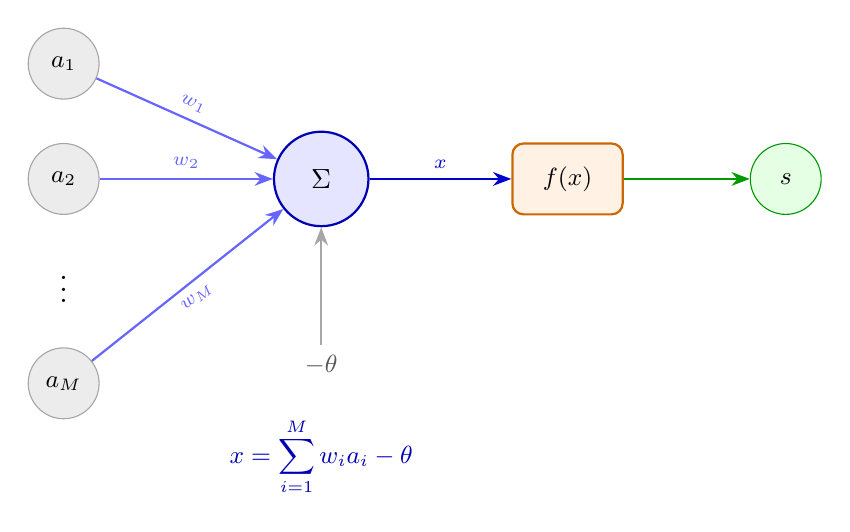
\begin{tikzpicture}[
  node distance=0.8cm and 1.6cm,
  inputnode/.style={circle, draw=gray!70, fill=gray!15, minimum size=0.9cm, font=\small},
  sumnode/.style={circle, draw=blue!70!black, fill=blue!10, minimum size=1.2cm,
                  font=\normalsize, thick},
  actnode/.style={rectangle, rounded corners=4pt, draw=orange!80!black,
                  fill=orange!10, minimum width=1.4cm, minimum height=0.9cm,
                  font=\small, thick},
  outnode/.style={circle, draw=green!60!black, fill=green!10,
                  minimum size=0.9cm, font=\small},
  >=Stealth
]

% Input nodes
\node[inputnode] (a1) {$a_1$};
\node[inputnode, below=0.55cm of a1] (a2) {$a_2$};
\node[below=0.45cm of a2, font=\large] (dots) {$\vdots$};
\node[inputnode, below=0.45cm of dots] (am) {$a_M$};

% Summation node
\node[sumnode, right=2.2cm of a2] (sum) {$\Sigma$};

% Activation node
\node[actnode, right=1.8cm of sum] (act) {$f(x)$};

% Output
\node[outnode, right=1.6cm of act] (out) {$s$};

% Bias
\node[below=1.5cm of sum, font=\small, text=gray!70!black] (bias) {$-\theta$};

% Arrows: inputs to sum
\draw[->, thick, blue!60] (a1) -- node[above, sloped, font=\scriptsize] {$w_1$} (sum);
\draw[->, thick, blue!60] (a2) -- node[above, sloped, font=\scriptsize] {$w_2$} (sum);
\draw[->, thick, blue!60] (am) -- node[below, sloped, font=\scriptsize] {$w_M$} (sum);

% Bias arrow
\draw[->, thick, gray!70] (bias) -- (sum);

% Sum to activation
\draw[->, thick, blue!80!black] (sum) -- node[above, font=\scriptsize] {$x$} (act);

% Activation to output
\draw[->, thick, green!60!black] (act) -- (out);

% Label the summation equation below the figure
\node[below=2.3cm of sum, font=\small, text=blue!70!black]
  {$x = \displaystyle\sum_{i=1}^{M} w_i a_i - \theta$};

\end{tikzpicture}
\caption{McCulloch--Pitts neuron model.
         $M$ weighted inputs are summed and the bias $\theta$ is subtracted
         to form the activation value $x$, which is then passed through a
         non-linear output function $f(\cdot)$ to produce the output $s$.}
\label{fig:mp-neuron}
\end{figure}

\subsection{Limitations of the MP Model}
\label{subsec:mp-limits}

\begin{warningbox}[title=Critical Limitation of the MP Model]
The MP model assumes \textbf{fixed weights}.
There is no mechanism for the model to \emph{learn} the weight values
from data.
Weights must be computed or assigned manually before use -- a serious
practical obstacle when the number of inputs and neurons grows large.
\end{warningbox}

This limitation motivated Rosenblatt's seminal advance: a model that
\emph{automatically adjusts} its weights in response to prediction
errors, introducing \emph{learning} into the computational neuron.

%=============================================================
\section{Learning Laws and the Perceptron}
\label{sec:perceptron}
%=============================================================

\subsection{The General Weight-Update Principle}
\label{subsec:weight-update}

All neural-network learning algorithms share a common skeleton:
at time step $t$, compute an incremental change $\Delta w_i(t)$ and
add it to the current weight:

\begin{equation}
  w_i(t+1) = w_i(t) + \Delta w_i(t)
  \label{eq:weight-update}
\end{equation}

The specific rule for computing $\Delta w_i(t)$ defines the
\emph{learning law}.
Common examples include: Hebb's law, the Perceptron learning law,
the Delta (Widrow--Hoff LMS) law, the correlation law, and the
instar/outstar laws.

\subsection{Rosenblatt's Perceptron Model}
\label{subsec:perceptron-model}

Frank Rosenblatt (1958) introduced the Perceptron as the first model
that could \emph{automatically learn} its weight parameters from labelled
examples.
The architecture retains the MP neuron equations (\cref{eq:activation,eq:output})
but adds an error-driven weight-update rule.

\begin{definition}[Perceptron Learning Rule]
\label{def:perceptron-rule}
Given a target output $b$ and actual output $s = f(x)$, define the
\textbf{error signal}:
\begin{equation}
  \delta = b - s
  \label{eq:error}
\end{equation}
The weight update for the $i$-th input connection is:
\begin{equation}
  \Delta w_i = \eta\,\delta\,a_i
  \label{eq:delta-w}
\end{equation}
where $\eta > 0$ is the \textbf{learning rate}.
The updated weight is:
\begin{equation}
  w_i(t+1) = w_i(t) + \eta\,\delta\,a_i
  \label{eq:update-rule}
\end{equation}
\end{definition}

\subsubsection{Effect of the Error Signal}
\label{subsubsec:error-effect}

\Cref{tab:error-cases} shows the three possible cases for $\delta$ and
the resulting effect on the weights.

\begin{table}[ht]
\centering
\caption{Perceptron weight-update cases based on the error $\delta = b - s$}
\label{tab:error-cases}
\begin{tabular}{cccp{6.5cm}}
\toprule
\textbf{Actual} $s$ & \textbf{Target} $b$ & $\delta$ & \textbf{Effect on weights} \\
\midrule
$s = b$  & --  & $0$  & No update; current weights are correct for this sample \\
$0$      & $1$ & $+1$ & Increase weights connected to active inputs (push activation up) \\
$1$      & $0$ & $-1$ & Decrease weights connected to active inputs (push activation down) \\
\bottomrule
\end{tabular}
\end{table}

\subsection{The Discrete Perceptron Learning Law}
\label{subsec:discrete-perceptron}

In the formal statement used in the course slides, the Perceptron
learning law is written using the sign function:

\begin{align}
  \Delta w_i &= \eta\bigl[b_i - \sgn(\vect{w}_i^T \vect{a})\bigr]\,a
  \label{eq:discrete-law-1}\\
  \Delta w_{ij} &= \eta\bigl[b_j - \sgn(\vect{w}_i^T \vect{a})\bigr]\,a_j,
    \quad j = 1, 2, \ldots, M
  \label{eq:discrete-law-2}
\end{align}

Key properties of the Perceptron learning law:
\begin{itemize}
  \item Weights are adjusted \emph{only} when the actual output $s_j$
        is incorrect.
  \item Weights are initialised to small random values prior to learning.
  \item It is a \textbf{supervised learning} algorithm: it requires a
        desired (target) output for each input.
  \item \textbf{Weights converge to final values by repeated use of
        input--output pairs.}
  \item The learning rate $\eta \ll 1$ is kept small to ensure stable
        error-corrective updates.
\end{itemize}

\begin{keyinsight}[title=The Breakthrough of Learning]
Before Rosenblatt's Perceptron, weights were fixed and had to be set
manually.
The Perceptron demonstrated for the first time that a neural unit could
\emph{automatically learn} its weights from data.
This was a foundational result in the history of artificial intelligence.
From the lecture: ``The concept of learning was demonstrated for the
first time in the neural network history. That's why this is treated as
one of the breakthrough results.''
\end{keyinsight}

%=============================================================
\section{Perceptron Working: Numerical Examples}
\label{sec:perceptron-examples}
%=============================================================

\subsection{Forward Pass Without Bias}
\label{subsec:no-bias}

Consider a three-input perceptron with the following values:

\begin{center}
\begin{tabular}{llll}
\toprule
\textbf{Input} & $x_1 = 0.2$ & $x_2 = 0.4$ & $x_3 = 0.6$ \\
\textbf{Weight} & $w_1 = -0.3$ & $w_2 = 0.4$ & $w_3 = -0.8$ \\
\bottomrule
\end{tabular}
\end{center}

The weighted sum is:
\begin{align}
  \sum_{i=1}^{3} w_i x_i
    &= (0.2)(-0.3) + (0.4)(0.4) + (0.6)(-0.8) \notag \\
    &= -0.06 + 0.16 - 0.48 \notag \\
    &= -0.38
  \label{eq:ws-no-bias}
\end{align}

Applying the step function: $f(-0.38) = \mathbf{0}$, since $-0.38 \leq 0$.

\subsection{Forward Pass With Bias}
\label{subsec:with-bias}

Using the same inputs and weights but adding a bias $b = 0.5$:
\begin{align}
  \sum_{i=1}^{3} w_i x_i + b
    &= -0.38 + 0.5 \notag \\
    &= 0.12
  \label{eq:ws-bias}
\end{align}

Applying the step function: $f(0.12) = \mathbf{1}$, since $0.12 > 0$.

\begin{example}[title=Impact of the Bias Term]
Adding a bias of $b = 0.5$ flipped the output from $0$ to $1$.
The bias acts as a learnable threshold that shifts the decision boundary
away from the origin.
\textbf{Without bias, the decision boundary must pass through the origin},
severely restricting which patterns can be classified correctly.
\end{example}

\subsection{Perceptron Architecture Diagram (With Bias)}
\label{subsec:perceptron-arch-diagram}

\begin{figure}[ht]
\centering
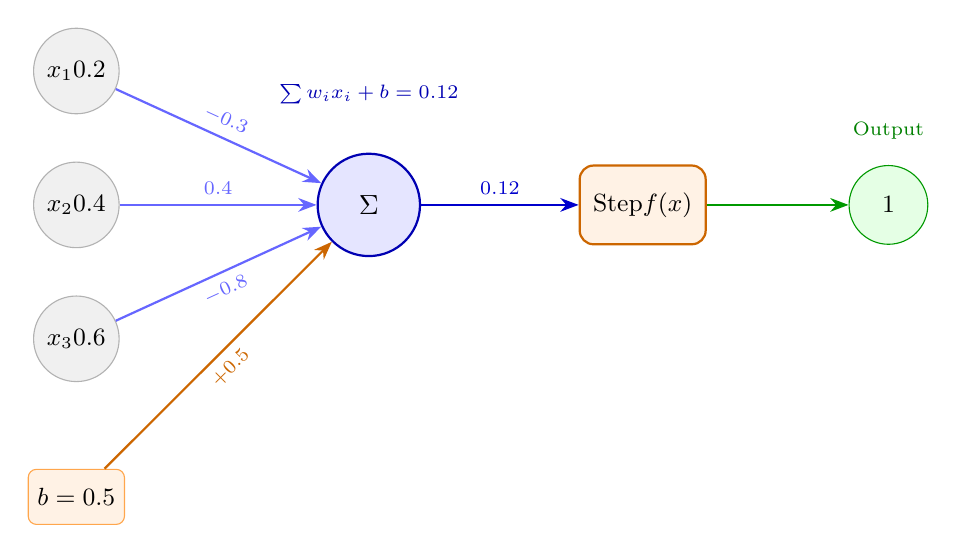
\begin{tikzpicture}[
  node distance=0.9cm and 2.0cm,
  inputnode/.style={circle, draw=gray!60, fill=gray!12, minimum size=1.0cm, font=\small},
  biasnode/.style={rectangle, rounded corners=3pt, draw=orange!70, fill=orange!10,
                   minimum width=1.1cm, minimum height=0.7cm, font=\small},
  sumnode/.style={circle, draw=blue!70!black, fill=blue!10, minimum size=1.3cm,
                  font=\normalsize, thick},
  actnode/.style={rectangle, rounded corners=5pt, draw=orange!80!black,
                  fill=orange!10, minimum width=1.6cm, minimum height=1.0cm,
                  font=\small, thick},
  outnode/.style={circle, draw=green!60!black, fill=green!10,
                  minimum size=1.0cm, font=\small\bfseries},
  >=Stealth
]

% Input nodes
\node[inputnode] (x1) {$x_1$\\$0.2$};
\node[inputnode, below=0.6cm of x1] (x2) {$x_2$\\$0.4$};
\node[inputnode, below=0.6cm of x2] (x3) {$x_3$\\$0.6$};

% Bias node
\node[biasnode, below=1.1cm of x3] (bias) {$b=0.5$};

% Summation node
\node[sumnode, right=2.5cm of x2] (sum) {$\Sigma$};

% Activation function node
\node[actnode, right=2.0cm of sum] (act) {Step\\$f(x)$};

% Output node
\node[outnode, right=1.8cm of act] (out) {$1$};

% Arrows
\draw[->, thick, blue!60] (x1) -- node[above, sloped, font=\scriptsize] {$-0.3$} (sum);
\draw[->, thick, blue!60] (x2) -- node[above, font=\scriptsize] {$0.4$} (sum);
\draw[->, thick, blue!60] (x3) -- node[below, sloped, font=\scriptsize] {$-0.8$} (sum);
\draw[->, thick, orange!80!black] (bias) -- node[below, sloped, font=\scriptsize] {$+0.5$} (sum);
\draw[->, thick, blue!80!black] (sum) -- node[above, font=\scriptsize] {$0.12$} (act);
\draw[->, thick, green!60!black] (act) -- (out);

% Annotation
\node[above=0.2cm of out, font=\scriptsize, text=green!50!black] {Output};
\node[above=0.5cm of sum, font=\scriptsize, text=blue!70!black] {$\sum w_i x_i + b = 0.12$};

\end{tikzpicture}
\caption{Perceptron with bias.
         The three weighted inputs sum to $-0.38$; adding bias $b=0.5$ gives
         $0.12$, which crosses the threshold to produce output $1$.}
\label{fig:perceptron-bias}
\end{figure}

\subsection{PyTorch Implementation}
\label{subsec:pytorch-impl}

The following PyTorch code (demonstrated live in Google Colab during
the session) replicates both forward-pass computations:

\begin{lstlisting}[style=python, caption={Perceptron forward pass in PyTorch (V13 -- 00:30:00)}, label={lst:forward-pass}]
import torch

# Inputs and weights
x = torch.tensor([0.2, 0.4, 0.6])
weights = torch.tensor([-0.3, 0.4, -0.8])

# Weighted sum (no bias)
weighted_sum = torch.dot(weights, x)   # tensor(-0.3800)

# Step activation function
def step_function(z):
    return 1 if z >= 0 else 0

output = step_function(weighted_sum)              # 0

# With bias b = 0.5
bias = 0.5
output_with_bias = step_function(weighted_sum + bias)  # 1
print(f"Without bias: {output}")         # 0
print(f"With bias:    {output_with_bias}")  # 1
\end{lstlisting}

%=============================================================
\section{Learning a Decision Boundary -- The Perceptron Trick}
\label{sec:decision-boundary}
%=============================================================

\subsection{Problem Setup: Placement Prediction}
\label{subsec:placement-problem}

The session uses a toy placement-prediction dataset to motivate the
Perceptron Trick.
Each student is described by two features -- CGPA ($x_1$) and IQ
($x_2$, scaled to IQ/10) -- and labelled with a binary placement
outcome ($y \in \{0, 1\}$).

\begin{table}[ht]
\centering
\caption{Placement dataset used in the Perceptron Trick demonstration}
\label{tab:placement}
\begin{tabular}{cccc}
\toprule
\textbf{Student} & \textbf{CGPA} ($x_1$) & \textbf{IQ/10} ($x_2$) & \textbf{Placed?} ($y$) \\
\midrule
1 & 6.5  & 11.0 & 0 (Not placed) \\
2 & 7.2  & 12.0 & 1 (Placed) \\
3 & 8.0  & 10.5 & 1 (Placed) \\
\bottomrule
\end{tabular}
\end{table}

\subsection{The Decision Boundary Equation}
\label{subsec:db-equation}

A perceptron with bias weight $w_0$ and feature weights $w_1, w_2$
classifies a point $(x_1, x_2)$ by the sign of:
\begin{equation}
  z = w_0 x_0 + w_1 x_1 + w_2 x_2, \qquad x_0 = 1 \text{ (bias input)}
  \label{eq:linear-combination}
\end{equation}

The \textbf{decision boundary} is the set of points where $z = 0$:
\begin{equation}
  w_0 + w_1 x_1 + w_2 x_2 = 0
  \label{eq:decision-boundary}
\end{equation}

Solving for $x_2$ gives the boundary line in feature space:
\begin{equation}
  x_2 = -\frac{w_0 + w_1 x_1}{w_2}
  \label{eq:boundary-line}
\end{equation}

\subsection{Numerical Derivation with Initial Weights}
\label{subsec:numerical-db}

Starting with random initial weights $w_0 = -1,\ w_1 = 0.5,\ w_2 = -0.3$:

\begin{align}
  -1 + 0.5\,x_1 - 0.3\,x_2 &= 0 \notag \\
  -0.3\,x_2 &= 1 - 0.5\,x_1 \notag \\
  x_2 &= \frac{1 - 0.5\,x_1}{-0.3} \notag \\
  x_2 &= -3.333 + 1.6\overline{6}\,x_1
  \label{eq:initial-boundary}
\end{align}

\begin{keyinsight}[title=Geometric Interpretation]
The decision boundary in \cref{eq:decision-boundary} is a hyperplane
in the $M$-dimensional feature space.
In two dimensions it is a straight line.
Points on one side are predicted as class 1; points on the other side
as class 0.
The Perceptron Trick iteratively rotates and translates this line until
all training points are correctly classified.
\end{keyinsight}

\subsection{The Perceptron Trick Algorithm}
\label{subsec:perceptron-trick}

The key intuition is: if a point is \emph{misclassified}, adjust the
weights so that the decision boundary moves towards the misclassified
point.

\begin{algorithm}[H]
\caption{Perceptron Learning (Perceptron Trick)}
\label{alg:perceptron-trick}
\SetAlgoLined
\DontPrintSemicolon
\KwIn{Training set $\{(\vect{x}^{(k)}, y^{(k)})\}_{k=1}^{N}$,
      learning rate $\eta$, max epochs $T$}
\KwOut{Weight vector $\vect{w} = (w_0, w_1, \ldots, w_n)^T$}
\BlankLine

\textbf{Initialise:} Set $x_0 \leftarrow 1$ (bias input)\;
\textbf{Initialise:} $w_i \leftarrow$ small random values, $i = 0, 1, \ldots, n$\;
\BlankLine

\For{$\text{epoch} = 1$ \KwTo $T$}{
  \For{each training example $(\vect{x}^{(k)}, y^{(k)})$}{
    Compute weighted sum: $z \leftarrow \sum_{i=0}^{n} w_i x_i^{(k)}$\;
    \BlankLine
    Predict output:
    $\hat{y} \leftarrow \begin{cases} 1 & \text{if } z \geq 0 \\ 0 & \text{if } z < 0 \end{cases}$\;
    \BlankLine
    Compute error: $e \leftarrow y^{(k)} - \hat{y}$\;
    \BlankLine
    \If{$e \neq 0$ \textup{(misclassification)}}{
      \For{$i = 0, 1, \ldots, n$}{
        $w_i \leftarrow w_i + \eta \cdot e \cdot x_i^{(k)}$
        \tcp*{Shift boundary toward point}
      }
    }
  }
  \BlankLine
  \lIf{no misclassified points}{\textbf{break}}
}
\Return $\vect{w}$\;
\end{algorithm}

\subsection{Decision Boundary Evolution Diagram}
\label{subsec:db-evolution}

\Cref{fig:db-evolution} illustrates how the decision boundary rotates
across training epochs on the placement dataset.

\begin{figure}[ht]
\centering
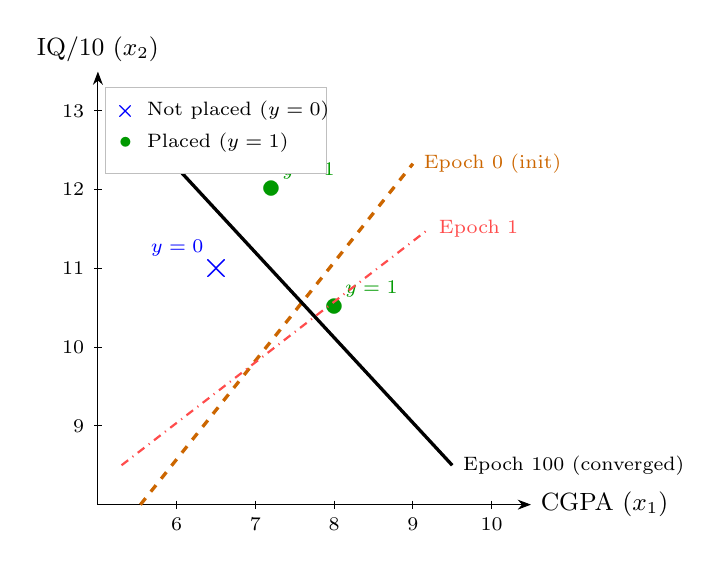
\begin{tikzpicture}[scale=1.0, >=Stealth]

% Axes
\draw[->] (0,0) -- (5.5,0) node[right, font=\small] {CGPA ($x_1$)};
\draw[->] (0,0) -- (0,5.5) node[above, font=\small] {IQ/10 ($x_2$)};

% Axis ticks and labels
\foreach \x/\xl in {1/6,2/7,3/8,4/9,5/10}{
  \draw (\x,0.05) -- (\x,-0.05) node[below, font=\scriptsize] {\xl};
}
\foreach \y/\yl in {1/9,2/10,3/11,4/12,5/13}{
  \draw (0.05,\y) -- (-0.05,\y) node[left, font=\scriptsize] {\yl};
}

% Class-0 point: CGPA=6.5 -> x=1.5, IQ/10=11.0 -> y=3.0
\node[blue, font=\Large] at (1.5,3.0) {\texttimes};
\node[blue, font=\scriptsize, above left=0.05cm] at (1.5,3.0) {$y=0$};

% Class-1 points: CGPA=7.2 -> x=2.2, IQ/10=12.0 -> y=4.0
\node[green!60!black, font=\Large] at (2.2,4.0) {$\bullet$};
\node[green!60!black, font=\scriptsize, above right=0.02cm] at (2.2,4.0) {$y=1$};

% CGPA=8.0 -> x=3.0, IQ/10=10.5 -> y=2.5
\node[green!60!black, font=\Large] at (3.0,2.5) {$\bullet$};
\node[green!60!black, font=\scriptsize, above right=0.02cm] at (3.0,2.5) {$y=1$};

% Initial decision boundary (epoch 0): x2 = -3.333 + 1.667*x1
% At x1=6 (plot-x=1): x2 = -3.333 + 10 = 6.667 (plot-y=6.667-9=-2.333) -- off plot
% Use parametric: x_plot = x1-6, y_plot = x2-9
% x2 = -3.333 + 1.667*x1; at x1=6: x2=6.667; at x1=10: x2=13.333
% plot-x=x1-6, plot-y=x2-9
% x1=6->plot_x=0, x2=6.667->plot_y=-2.33 (clamp to 0)
% x1=6.54->x2=9 so plot_x=0.54, plot_y=0
% x1=10->plot_x=4, plot_y=4.33
\draw[orange!80!black, dashed, very thick]
  (0.54,0) -- (4.0,4.33)
  node[right, font=\scriptsize, orange!80!black] {Epoch 0 (init)};

% Epoch 1 boundary: slightly shifted
\draw[red!70, dashdotted, thick]
  (0.3,0.5) -- (4.2,3.5)
  node[right, font=\scriptsize, red!70] {Epoch 1};

% Final boundary (epoch 100): separates class 0 from class 1
\draw[black, very thick]
  (0.8,4.5) -- (4.5,0.5)
  node[right, font=\scriptsize] {Epoch 100 (converged)};

% Legend box
\begin{scope}[shift={(0.1,4.2)}]
  \draw[fill=white, draw=gray!50] (0,0) rectangle (2.8,1.1);
  \node[blue, font=\small] at (0.25,0.8) {\texttimes};
  \node[font=\scriptsize, right] at (0.4,0.8) {Not placed ($y=0$)};
  \node[green!60!black, font=\small] at (0.25,0.4) {$\bullet$};
  \node[font=\scriptsize, right] at (0.4,0.4) {Placed ($y=1$)};
\end{scope}

\end{tikzpicture}
\caption{Decision boundary evolution on the placement dataset.
         The boundary starts randomly (dashed orange), shifts after epoch~1
         (dash-dotted red), and converges to a clean separator at epoch~100
         (solid black).}
\label{fig:db-evolution}
\end{figure}

\subsection{Full PyTorch Training Loop}
\label{subsec:training-loop}

\begin{lstlisting}[style=python, caption={Full perceptron training loop with weight history (V20 -- 01:01:00)}, label={lst:training-loop}]
import torch

# Dataset: CGPA (x1), IQ/10 (x2), placement label
X_raw = torch.tensor([
    [6.5, 11.0],
    [7.2, 12.0],
    [8.0, 10.5],
], dtype=torch.float32)
Y = torch.tensor([0, 1, 1], dtype=torch.float32)

# Augment with bias column x0 = 1
bias_col = torch.ones(X_raw.shape[0], 1)
X = torch.cat([bias_col, X_raw], dim=1)   # shape (3, 3)

# Random weight initialisation: w0=-1, w1=0.5, w2=-0.3
W = torch.tensor([-1.0, 0.5, -0.3])

def predict(x_vec, w_vec):
    z = torch.dot(w_vec, x_vec)
    return 1 if z >= 0 else 0

eta = 0.1
epochs = 100
weight_history = []

for epoch in range(epochs):
    for i in range(len(X)):
        xi  = X[i]
        yi  = Y[i].item()
        y_hat = predict(xi, W)
        error = yi - y_hat
        if error != 0:
            W = W + eta * error * xi
    weight_history.append(W.clone())

W_epoch1  = weight_history[0]
W_epoch2  = weight_history[1]
W_final   = weight_history[-1]
print(f"Final weights: {W_final}")
\end{lstlisting}

\subsection{Weight History Across Training}
\label{subsec:weight-history}

\Cref{tab:weight-history} summarises how the three weight parameters
evolve during training.

\begin{table}[ht]
\centering
\caption{Weight evolution during perceptron training on the placement dataset}
\label{tab:weight-history}
\begin{tabular}{lccc}
\toprule
\textbf{Epoch} & $w_0$ (bias) & $w_1$ (CGPA) & $w_2$ (IQ/10) \\
\midrule
Initialisation & $-1.0$  & $0.5$  & $-0.3$  \\
Epoch 1        & shifts after first misclassification & updated & updated \\
Epoch 2        & further shift & further shift & further shift \\
$\vdots$       & $\vdots$ & $\vdots$ & $\vdots$ \\
Epoch $\leq 100$ & converged & converged & converged \\
\bottomrule
\multicolumn{4}{l}{\small Note: exact values vary per random seed.
Pattern: rapid changes in early epochs, stabilises once all} \\
\multicolumn{4}{l}{\small training points are correctly classified.} \\
\end{tabular}
\end{table}

%=============================================================
\section{The Perceptron Convergence Theorem}
\label{sec:convergence}
%=============================================================

\begin{theorem}[Perceptron Convergence Theorem]
\label{thm:perceptron-convergence}
If the training data is \textbf{linearly separable}, the perceptron
learning algorithm is guaranteed to converge -- that is, to find a
weight vector $\vect{w}^*$ that correctly classifies all training
examples -- in a \textbf{finite} number of weight updates.
\end{theorem}

\begin{remark}
\label{rem:convergence-finite}
The convergence theorem provides an upper bound on the number of
misclassifications before convergence, which depends on the margin
(the distance from the closest point to the separating hyperplane)
and the norm of the input vectors.
Specifically, if there exists a weight vector $\vect{w}^*$ with
$\|\vect{w}^*\| = 1$ such that $y^{(k)}(\vect{w}^{*T}\vect{x}^{(k)}) \geq \gamma$
for all $k$, the number of mistakes is at most $R^2/\gamma^2$ where
$R = \max_k \|\vect{x}^{(k)}\|$.
\end{remark}

\begin{keyinsight}[title=What the Convergence Theorem Does Not Guarantee]
The theorem guarantees convergence \emph{only when the data is linearly
separable}.
For non-linearly-separable data (e.g., XOR), the algorithm will never
converge -- the weights oscillate indefinitely.
Moreover, even when the data is linearly separable, the converged
solution is not necessarily optimal: there can be \emph{infinitely
many} valid separating hyperplanes.
\end{keyinsight}

%=============================================================
\section{Perceptron Representation Problem}
\label{sec:representation}
%=============================================================

\subsection{Linear Separability}
\label{subsec:linear-separability}

A binary classification problem on inputs $\{0, 1\}^M$ is
\textbf{linearly separable} if there exists a hyperplane
$\vect{w}^T \vect{x} = 0$ such that all class-1 points lie on one
side and all class-0 points on the other.

For $M = 2$ binary inputs there are $2^{2^M} = 2^4 = 16$ distinct
Boolean functions.
Of these 16 functions, only \textbf{14 are linearly separable}.

\begin{example}[title=Linearly Separable Boolean Functions]
The following two-input functions are linearly separable:
AND, OR, NOT, NOR, NAND, and their combinations.
Each can be implemented by a single-layer perceptron.
\end{example}

\subsection{The XOR Problem}
\label{subsec:xor}

XOR (exclusive-or) is the canonical example of a \emph{non-linearly
separable} function.
\Cref{tab:xor-truth} shows the truth table.

\begin{table}[ht]
\centering
\caption{XOR truth table showing non-linear separability}
\label{tab:xor-truth}
\begin{tabular}{ccc}
\toprule
$A$ & $B$ & $A \oplus B$ \\
\midrule
0 & 0 & 0 \\
0 & 1 & 1 \\
1 & 0 & 1 \\
1 & 1 & 0 \\
\bottomrule
\end{tabular}
\end{table}

No single straight line can separate the output-1 points
$\{(0,1),\,(1,0)\}$ from the output-0 points $\{(0,0),\,(1,1)\}$
in the unit square.
XNOR (the complement of XOR) is equally non-separable.

\subsection{Hard Problems}
\label{subsec:hard-problems}

Problems that are not linearly separable are called \textbf{hard
problems} for a single-layer perceptron.

\begin{definition}[Hard Problem]
\label{def:hard-problem}
A pattern classification problem is called a \textbf{hard problem} if
it is not representable by a single-layer perceptron -- i.e., the
classes are not linearly separable, and the perceptron learning
algorithm will not converge on it.
\end{definition}

As the input dimensionality $M$ increases, the fraction of Boolean
functions that are linearly separable decreases rapidly.
This means the single-layer perceptron becomes increasingly limited
as problems grow in complexity.

\begin{warningbox}[title=Practical Implication]
Real-world data (images, speech, text) is almost never linearly
separable in the raw input space.
Relying solely on a single-layer perceptron for such tasks will result
in the algorithm failing to converge and producing poor classifiers.
A deeper architecture is required.
\end{warningbox}

%=============================================================
\section{Beyond the Perceptron: Multilayer Networks}
\label{sec:mlp}
%=============================================================

\subsection{Two-Layer Networks: Convex Regions}
\label{subsec:two-layer}

Adding a \emph{single hidden layer} to the perceptron allows the
network to form \textbf{convex decision regions}.

\begin{definition}[Convex Region]
\label{def:convex}
A region $\mathcal{R} \subseteq \R^M$ is \textbf{convex} if, for any
two points $\vect{p}, \vect{q} \in \mathcal{R}$, the entire line
segment $\lambda\vect{p} + (1-\lambda)\vect{q}$ for
$\lambda \in [0,1]$ lies within $\mathcal{R}$.
\end{definition}

Each hidden-layer unit contributes one half-space boundary.
The intersection of these half-spaces forms a convex region.
A two-layer network can therefore solve XOR by combining two
linear separators.

\subsection{Three-Layer Networks: Arbitrary Regions}
\label{subsec:three-layer}

A second hidden layer (three layers total) can form the
\textbf{union of convex regions}, thereby approximating
\emph{any} finite binary classification boundary.
The shape and size of the class regions depend on the number of
hidden units in each layer.

\subsection{Four-Layer Networks: Full Generality}
\label{subsec:four-layer}

A four-layer network (input + three layers of nonlinear units)
can perform \textbf{any complex pattern classification} task.
This is the Multilayer Perceptron (MLP), also called a
feedforward fully-connected network.

\subsection{Network Capability Summary}
\label{subsec:network-summary}

\Cref{tab:network-capability} and \cref{fig:mlp-progression} compare
the representational power of increasingly deep perceptron networks.

\begin{table}[ht]
\centering
\caption{Decision region capability as a function of network depth}
\label{tab:network-capability}
\begin{tabularx}{\textwidth}{lllX}
\toprule
\textbf{Network}         & \textbf{Hidden Layers} & \textbf{Decision Region} & \textbf{Example Problems} \\
\midrule
1-layer perceptron       & 0 & Hyperplane (linear only) & AND, OR, NOT \\
2-layer (1 hidden layer) & 1 & Convex region            & XOR, bounded convex shapes \\
3-layer (2 hidden layers)& 2 & Arbitrary (non-convex)   & Any finite binary task \\
4-layer (3 hidden layers)& 3 & Any complex pattern      & General classification \\
\bottomrule
\end{tabularx}
\end{table}

\begin{figure}[ht]
\centering
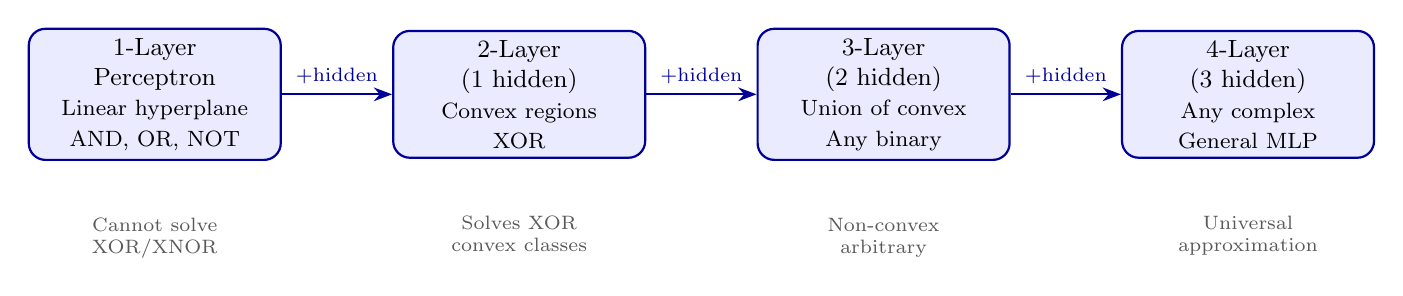
\begin{tikzpicture}[
  block/.style={rectangle, rounded corners=6pt, draw=blue!60!black,
                fill=blue!8, minimum width=3.2cm, minimum height=1.6cm,
                align=center, font=\small, thick},
  arrow/.style={->, thick, blue!60!black},
  label/.style={font=\scriptsize, text=gray!70!black, align=center},
  >=Stealth,
  node distance=1.2cm
]

\node[block] (L1) {1-Layer\\Perceptron\\{\footnotesize Linear hyperplane}\\{\footnotesize AND, OR, NOT}};
\node[block, right=1.4cm of L1] (L2) {2-Layer\\(1 hidden)\\{\footnotesize Convex regions}\\{\footnotesize XOR}};
\node[block, right=1.4cm of L2] (L3) {3-Layer\\(2 hidden)\\{\footnotesize Union of convex}\\{\footnotesize Any binary}};
\node[block, right=1.4cm of L3] (L4) {4-Layer\\(3 hidden)\\{\footnotesize Any complex}\\{\footnotesize General MLP}};

\draw[arrow] (L1) -- node[above, font=\scriptsize] {+hidden} (L2);
\draw[arrow] (L2) -- node[above, font=\scriptsize] {+hidden} (L3);
\draw[arrow] (L3) -- node[above, font=\scriptsize] {+hidden} (L4);

% Capability labels below
\node[label, below=0.6cm of L1] {Cannot solve\\XOR/XNOR};
\node[label, below=0.6cm of L2] {Solves XOR\\convex classes};
\node[label, below=0.6cm of L3] {Non-convex\\arbitrary};
\node[label, below=0.6cm of L4] {Universal\\approximation};

\end{tikzpicture}
\caption{Progression of representational power as hidden layers are added.
         Each additional layer unlocks a more expressive class of decision
         boundaries, culminating in the universal approximation capability
         of deep MLPs.}
\label{fig:mlp-progression}
\end{figure}

\subsection{The Problem of Multiple Solutions}
\label{subsec:multiple-solutions}

Even when the data is linearly separable, the Perceptron Trick finds
\emph{some} valid hyperplane -- but there may be infinitely many such
hyperplanes.
The algorithm has no notion of which separator is ``best.''
This motivates later techniques:

\begin{itemize}
  \item \textbf{Support Vector Machines} -- find the maximum-margin
        separator (widest possible gap between classes).
  \item \textbf{Backpropagation + gradient descent} -- optimise a
        smooth loss function over all weights simultaneously in MLPs.
\end{itemize}

\begin{keyinsight}[title=From Perceptron to Deep Learning]
The Perceptron established the foundational idea that neural units can
learn from data.
Its limitation -- inability to solve non-linearly-separable problems
-- directly motivated the development of multilayer networks.
These, combined with the backpropagation algorithm (introduced in later
sessions), form the basis of all modern deep learning systems.
\end{keyinsight}

%=============================================================
\section{Topology and Network Organisation}
\label{sec:topology}
%=============================================================

The term \textbf{topology} refers to how neurons are organised and
connected within a network.
Key design choices include:

\begin{enumerate}[label=(\alph*)]
  \item \textbf{Layer structure:} All neurons in a layer share the same
        activation dynamics and output function.
  \item \textbf{Connection type:}
        \begin{itemize}
          \item \emph{Interlayer connections} -- between adjacent layers
                (standard feedforward).
          \item \emph{Intralayer connections} -- within a layer
                (as in Hopfield networks).
          \item \emph{Both} -- recurrent networks.
        \end{itemize}
  \item \textbf{Information flow:}
        \begin{itemize}
          \item \emph{Feedforward} -- information flows from input to
                output only.
          \item \emph{Feedback (recurrent)} -- outputs feed back to
                earlier layers.
          \item \emph{Both} -- hybrid architectures.
        \end{itemize}
\end{enumerate}

\begin{remark}
\label{rem:power-of-layers}
The real power of neural networks does not come from the complexity
of individual neurons.
From the lecture: ``\ldots the strength or the efficiency of these neural
network or deep learning models in terms of modeling the information
comes because of the layered networks of these neurons in the form of
layers.''
\end{remark}

%=============================================================
\section{Summary and Conclusions}
\label{sec:summary}
%=============================================================

\subsection{Session Highlights}
\label{subsec:highlights}

Session~03 covered the complete arc from fixed mathematical neuron
models to trainable classifiers and their limits.
The key results are summarised below.

\subsubsection*{McCulloch--Pitts Model (1943)}
\begin{itemize}
  \item First mathematical model of an artificial neuron.
  \item Computes $x = \sum_{i=1}^{M} w_i a_i - \theta$ and outputs
        $s = f(x)$ via a binary non-linear function.
  \item \textbf{Limitation:} fixed weights, no learning capability.
\end{itemize}

\subsubsection*{Rosenblatt's Perceptron (1958)}
\begin{itemize}
  \item Extends MP neuron with the error-driven update rule
        $\Delta w_i = \eta(b - s)a_i$.
  \item First demonstration of \emph{learning} in a neural unit.
  \item Converges in finite steps for linearly separable data
        (Perceptron Convergence Theorem).
  \item \textbf{Limitation:} cannot represent non-linearly-separable
        functions (e.g., XOR, XNOR).
\end{itemize}

\subsubsection*{The Perceptron Trick}
\begin{itemize}
  \item For each misclassified point, shift the decision boundary
        toward it: $w_i \leftarrow w_i + \eta \cdot e \cdot x_i$.
  \item Works geometrically: each update rotates/translates the
        separating hyperplane to reduce error.
  \item Demonstrated live on the CGPA/IQ placement dataset in PyTorch.
\end{itemize}

\subsubsection*{Multilayer Perceptrons}
\begin{itemize}
  \item Adding hidden layers increases representational power.
  \item 1 hidden layer $\Rightarrow$ convex decision regions (solves XOR).
  \item 2 hidden layers $\Rightarrow$ arbitrary decision regions.
  \item 3 hidden layers (4-layer network) $\Rightarrow$ universal
        pattern classification.
\end{itemize}

\subsection{Key Equations Reference}
\label{subsec:equations}

\begin{align}
  \text{Activation:} \quad
    x &= \sum_{i=1}^{M} w_i\,a_i - \theta \tag{MP activation}\\
  \text{Output:} \quad
    s &= f(x) \tag{neuron output}\\
  \text{Error:} \quad
    \delta &= b - s \tag{Perceptron error}\\
  \text{Weight update:} \quad
    \Delta w_i &= \eta\,\delta\,a_i \tag{Perceptron rule}\\
  \text{Recursive update:} \quad
    w_i(t+1) &= w_i(t) + \Delta w_i(t) \tag{weight dynamics}\\
  \text{Decision boundary:} \quad
    x_2 &= -\frac{w_0 + w_1 x_1}{w_2} \tag{boundary line}
\end{align}

\subsection{Looking Ahead}
\label{subsec:looking-ahead}

Session~04 will introduce the \textbf{Multi-Layer Perceptron} in detail,
addressing the following open questions from this session:
\begin{enumerate}
  \item How do we train hidden-layer weights that have no direct
        target labels? (Answer: backpropagation.)
  \item Which specific non-linear activation functions are most useful
        in deep networks? (Answer: ReLU, sigmoid, tanh -- universal
        approximation theorem.)
  \item How do we choose the best separating hyperplane among all valid
        ones? (Answer: Support Vector Machines, maximum margin.)
\end{enumerate}

\vspace{1em}
\begin{tcolorbox}[colback=gray!5, colframe=gray!50!black,
  title={\bfseries Session 03 -- Quick Reference Card}]
\begin{center}
\begin{tabular}{ll}
\toprule
\textbf{Model} & \textbf{Key property} \\
\midrule
McCulloch--Pitts & Fixed weights, first mathematical neuron \\
Perceptron & Error-driven learning, linear boundary \\
2-layer MLP & Convex decision regions, solves XOR \\
$\geq$3-layer MLP & Universal approximation \\
\midrule
\textbf{Symbol} & \textbf{Meaning} \\
\midrule
$\eta$ & Learning rate ($0 < \eta \ll 1$) \\
$\delta = b - s$ & Perceptron error signal \\
$\Delta w_i = \eta\,\delta\,a_i$ & Weight update \\
$w_0$ & Bias weight ($x_0 = 1$) \\
\bottomrule
\end{tabular}
\end{center}
\end{tcolorbox}

%=============================================================

\clearpage

%% ============================================================
%% Session 04: Perceptron: Bias, Convergence Theorem, Linear Separability, and MLP Motivation
%% ============================================================
\part{Session 04: Perceptron: Bias, Convergence Theorem, Linear Separability, and MLP Motivation}

%% ══════════════════════════════════════════════════════════════════════
%%  TITLE PAGE
%% ══════════════════════════════════════════════════════════════════════
\begin{titlepage}
  \centering
  \vspace*{2cm}
  {\Large\bfseries Deep Learning Course\par}
  \vspace{0.5cm}
  {\large IIIT Dharwad\par}
  \vspace{1.5cm}
  \rule{\linewidth}{0.5mm}\\[0.4cm]
  {\huge\bfseries Session 04\\[0.3cm]
   Perceptron: Bias, Convergence Theorem,\\
   Linear Separability, and MLP Motivation\par}
  \rule{\linewidth}{0.5mm}\\[1.5cm]

  \begin{tabular}{rl}
    \textbf{Session Number:} & 04 \\[4pt]
    \textbf{Slide Deck:}     & 03-DL-Perceptron (continuation) \\[4pt]
    \textbf{Duration:}       & 1 hour 47 minutes \\[4pt]
    \textbf{Instructors:}    & Prof.\ S R M Prasanna \& Dr.\ Sunil Saumya \\[4pt]
    \textbf{Institution:}    & IIIT Dharwad \\[4pt]
    \textbf{Video:}          & \url{https://vimeo.com/1141589945} \\[4pt]
  \end{tabular}

  \vfill
  {\large\itshape Lecture Notes compiled from video transcript and visual extractions\par}
\end{titlepage}

%% ══════════════════════════════════════════════════════════════════════
%%  TABLE OF CONTENTS
%% ══════════════════════════════════════════════════════════════════════

\newpage

%% ══════════════════════════════════════════════════════════════════════
\section{Introduction}
\label{sec:intro}
%% ══════════════════════════════════════════════════════════════════════

Session~04 continues directly from Session~03, completing the coverage of
the perceptron learning model before motivating the transition to
multi-layer networks.  The session was delivered by
Prof.\ S R M Prasanna and Dr.\ Sunil Saumya at IIIT Dharwad.

The lecture begins by revisiting the role of \emph{bias} in shifting the
perceptron's decision boundary and then states the \emph{Perceptron
Convergence Theorem}: for linearly separable data, the algorithm is
guaranteed to reach a finite set of separating weights.  This guarantee
evaporates for linearly inseparable problems such as XOR, motivating the
introduction of hidden layers and, ultimately, the \emph{Multi-Layer
Perceptron} (MLP).

A landmark result due to Lippmann (1987) -- reproduced in
B.~Yegnanarayana's textbook (1999) as Figure~4.10 -- formalises the
relationship between network depth and the complexity of the achievable
decision regions:
\begin{itemize}[noitemsep]
  \item A \emph{two-layer} network (single perceptron layer) partitions
        the input space with a linear hyperplane.
  \item A \emph{three-layer} network (one hidden layer) can form convex
        decision regions.
  \item A \emph{four-layer} network (two hidden layers) can form
        \emph{arbitrary} decision regions.
\end{itemize}

The session also introduces the principal activation functions used in
practice: step, sigmoid, tanh, and ReLU, and demonstrates experimentally
that a single perceptron solves AND/OR but fails on XOR.

\subsection{Session Roadmap}
\label{subsec:roadmap}

\Cref{sec:prereqs} reviews the mathematical prerequisites.
\Cref{sec:bias} explains the role of bias and the compact bias-as-weight
notation.  \Cref{sec:convergence} states and discusses the Convergence
Theorem together with binary and multiclass linear separability.
\Cref{sec:inseparable} covers linearly inseparable problems, the XOR
failure, and the depth-vs-region-complexity table.
\Cref{sec:mlp-motivation} motivates and defines the Multi-Layer
Perceptron.  \Cref{sec:activations} surveys the common activation
functions.  \Cref{sec:conclusion} summarises the key takeaways.

%% ══════════════════════════════════════════════════════════════════════
\section{Background and Prerequisites}
\label{sec:prereqs}
%% ══════════════════════════════════════════════════════════════════════

\subsection{The Perceptron Model}
\label{subsec:perceptron-model}

A perceptron with $n$ inputs $x_1, x_2, \ldots, x_n$, corresponding
weights $w_1, w_2, \ldots, w_n$, and bias $b$ computes:

\begin{equation}
  \label{eq:perceptron}
  y = f\!\left(\sum_{i=1}^{n} w_i x_i + b\right),
\end{equation}

where $f$ is the activation function.  In the classical formulation
$f$ is the Heaviside step function:

\begin{equation}
  \label{eq:step}
  f(z) =
  \begin{cases}
    1 & \text{if } z \geq 0, \\
    0 & \text{otherwise.}
  \end{cases}
\end{equation}

\subsection{Bias as an Augmented Weight}
\label{subsec:bias-weight}

A convenient notational trick absorbs the bias into the weight vector by
augmenting the input with a fixed component $x_0 = 1$ (some formulations
use $x_0 = -1$ when the threshold is subtracted):

\begin{equation}
  \label{eq:augmented}
  y = f\!\left(\sum_{i=0}^{n} w_i x_i\right), \quad x_0 \equiv 1,
  \quad w_0 \equiv b.
\end{equation}

This lets the learning rule treat $b$ on an equal footing with all other
weights; only $x_0$ is fixed -- its ``weight'' $w_0$ is learned from data.

\subsection{Perceptron Learning Rule}
\label{subsec:learning-rule}

For each training sample $(\mathbf{x}^{(k)}, d^{(k)})$ with desired
output $d^{(k)} \in \{0,1\}$, the update rule is:

\begin{equation}
  \label{eq:update}
  w_i \leftarrow w_i + \eta \bigl(d^{(k)} - y^{(k)}\bigr)\, x_i^{(k)},
  \quad i = 0, 1, \ldots, n,
\end{equation}

where $\eta > 0$ is the learning rate.  The update is non-zero only on
misclassified samples; correctly classified samples leave the weights
unchanged.

\begin{keyinsight}[title=Key Insight -- Weight Update on Misclassification Only]
The perceptron learning rule is a \emph{reactive} correction: it modifies
the weight vector only when the current boundary misclassifies a sample.
On correctly classified samples, $d^{(k)} - y^{(k)} = 0$ and no change
is made.  This property makes the algorithm efficient but also means that
the final boundary depends on the order in which samples are presented.
\end{keyinsight}

\subsection{Geometric Interpretation}
\label{subsec:geometry}

The decision boundary is the set of points satisfying:

\begin{equation}
  \label{eq:boundary}
  \sum_{i=0}^{n} w_i x_i = 0,
\end{equation}

which in two dimensions ($n = 2$) describes a straight line.  Solving
for $x_2$:

\begin{equation}
  \label{eq:line}
  x_2 = -\frac{w_0 + w_1 x_1}{w_2}.
\end{equation}

For every value of $x_1$ one obtains the corresponding $x_2$ on the
boundary, enabling a direct plot of the separating line.

%% ══════════════════════════════════════════════════════════════════════
\section{The Role of Bias and Working Example}
\label{sec:bias}
%% ══════════════════════════════════════════════════════════════════════

\subsection{Why Bias Matters}
\label{subsec:why-bias}

Without a bias term the decision boundary defined by
$\sum_i w_i x_i = 0$ must pass through the origin.  This severely
restricts the set of separable configurations.  The bias parameter $b$
(equivalently $w_0$) shifts the boundary away from the origin, enabling
the perceptron to classify patterns whose natural boundary does not
pass through the origin.

\begin{keyinsight}[title=Key Insight -- Bias Shifts the Decision Boundary]
Bias provides an extra degree of freedom equivalent to translating the
hyperplane.  It is a \emph{learned} parameter, updated by the same rule
as ordinary weights.  Without it, the model is restricted to boundaries
passing through the origin in the augmented input space.
\end{keyinsight}

\subsection{Numerical Example (V01)}
\label{subsec:bias-example}

Consider a three-input perceptron with the following values (from the
lecture slide at timestamp 00:21:44):

\[
  x_1 = 0.2,\quad x_2 = 0.4,\quad x_3 = 0.6,\quad b = 0.5
\]
\[
  w_1 = -0.3,\quad w_2 = 0.4,\quad w_3 = -0.8
\]

\textbf{Step 1: Weighted sum without bias.}
\begin{align}
  \label{eq:weighted-sum}
  \sum_{i=1}^{3} w_i x_i
    &= (0.2)(-0.3) + (0.4)(0.4) + (0.6)(-0.8) \notag \\
    &= -0.06 + 0.16 - 0.48 \notag \\
    &= -0.38.
\end{align}

\textbf{Step 2: Add bias.}
\begin{equation}
  \label{eq:add-bias}
  z = -0.38 + 0.5 = 0.12.
\end{equation}

\textbf{Step 3: Apply step function.}
\begin{equation}
  \label{eq:apply-step}
  y = f(0.12) = 1 \quad (\text{since } 0.12 \geq 0).
\end{equation}

\begin{example}[title=Example -- Effect of Bias on Classification]
Without the bias the net input would be $-0.38$, yielding $y = 0$.
Adding $b = 0.5$ shifts the value to $+0.12$, flipping the classification
to $y = 1$.  This illustrates that for patterns whose weighted sum falls
slightly below zero, a learnable bias can still produce the correct output.
\end{example}

\subsection{TikZ Diagram: Perceptron with Bias}
\label{subsec:tikz-bias}

\Cref{fig:perceptron-bias} shows the architecture corresponding to the
numerical example above.

\begin{figure}[ht]
\centering
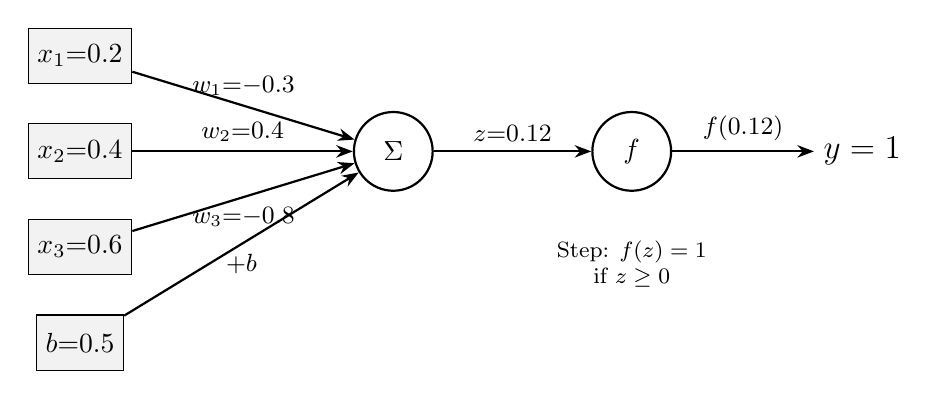
\begin{tikzpicture}[
    node distance=1.6cm and 2.4cm,
    neuron/.style={circle, draw, minimum size=1cm, thick},
    input/.style={rectangle, draw, minimum size=0.7cm, fill=gray!10},
    arr/.style={-{Stealth[length=6pt]}, thick},
    label style/.style={font=\small}
  ]

  %% Input nodes
  \node[input] (x1) {$x_1{=}0.2$};
  \node[input, below=0.5cm of x1] (x2) {$x_2{=}0.4$};
  \node[input, below=0.5cm of x2] (x3) {$x_3{=}0.6$};
  \node[input, below=0.5cm of x3] (b)  {$b{=}0.5$};

  %% Summation node
  \node[neuron, right=2.8cm of x2] (sum) {$\Sigma$};

  %% Activation node
  \node[neuron, right=2.0cm of sum] (act) {$f$};

  %% Output
  \node[right=1.8cm of act, font=\large\bfseries] (out) {$y = 1$};

  %% Arrows from inputs to sum
  \draw[arr] (x1) -- node[above, label style]{$w_1{=}{-}0.3$} (sum);
  \draw[arr] (x2) -- node[above, label style]{$w_2{=}0.4$}   (sum);
  \draw[arr] (x3) -- node[below, label style]{$w_3{=}{-}0.8$} (sum);
  \draw[arr] (b)  -- node[below, label style]{$+b$}           (sum);

  %% Sum to activation
  \draw[arr] (sum) -- node[above, label style]{$z{=}0.12$} (act);

  %% Activation to output
  \draw[arr] (act) -- node[above, label style]{$f(0.12)$} (out);

  %% Step function annotation
  \node[below=0.5cm of act, font=\footnotesize, align=center]
    {Step: $f(z)=1$\\if $z\geq 0$};

\end{tikzpicture}
\caption{Perceptron with bias: three inputs plus a bias unit feeding a
  summation node and a step-function activation.  The bias shifts the
  net input from $-0.38$ to $+0.12$, changing the output from 0 to 1.}
\label{fig:perceptron-bias}
\end{figure}

%% ══════════════════════════════════════════════════════════════════════
\section{Perceptron Convergence and Linear Separability}
\label{sec:convergence}
%% ══════════════════════════════════════════════════════════════════════

\subsection{The Perceptron Convergence Theorem}
\label{subsec:convergence-theorem}

\begin{theorem}[Perceptron Convergence Theorem]
\label{thm:convergence}
If the training data are linearly separable, then the perceptron learning
algorithm (\cref{eq:update}) converges after a finite number of weight
updates.  The resulting weight vector defines a linear hyperplane that
correctly separates all training samples.
\end{theorem}

\begin{remark}
\label{rem:uniqueness}
The theorem guarantees \emph{existence} of a separating hyperplane and
termination in \emph{finite steps}, but it does \emph{not} guarantee
uniqueness.  There may be infinitely many valid separating hyperplanes,
and the algorithm will stop at whichever one it reaches first, depending
on initialisation and sample ordering.
\end{remark}

\subsection{Linear Separability -- Definition}
\label{subsec:linear-separability-def}

\begin{definition}[Linear Separability]
\label{def:linsep}
A set of labelled data points
$\{(\mathbf{x}^{(k)}, d^{(k)})\}_{k=1}^{N}$ with $d^{(k)} \in \{-1, +1\}$
is \emph{linearly separable} if there exists a weight vector $\mathbf{w}$
and bias $b$ such that:
\begin{equation}
  \label{eq:linsep}
  d^{(k)}\!\left(\mathbf{w}^{\top}\mathbf{x}^{(k)} + b\right) > 0
  \quad \forall\, k.
\end{equation}
In two dimensions this means the two classes can be separated by a
straight line; in $M$ dimensions, by a hyperplane.
\end{definition}

\subsection{Boolean Functions and Linear Separability}
\label{subsec:boolean}

For $M = 2$ binary input variables there are $2^{2^M} = 2^4 = 16$
possible Boolean functions.  Of these, \textbf{14 are linearly separable}
and two are not.  \Cref{tab:boolean-gates} summarises the key cases.

\begin{table}[ht]
\centering
\caption{Linear separability of 2-input Boolean functions.}
\label{tab:boolean-gates}
\begin{tabular}{lcccc}
\toprule
\textbf{Function} & \textbf{(0,0)} & \textbf{(0,1)} & \textbf{(1,0)} & \textbf{(1,1)} \\
& output & output & output & output \\
\midrule
AND   & 0 & 0 & 0 & 1 \\
OR    & 0 & 1 & 1 & 1 \\
NAND  & 1 & 1 & 1 & 0 \\
NOR   & 1 & 0 & 0 & 0 \\
\midrule
\textbf{XOR}  & \textbf{0} & \textbf{1} & \textbf{1} & \textbf{0} \\
\textbf{XNOR} & \textbf{1} & \textbf{0} & \textbf{0} & \textbf{1} \\
\bottomrule
\end{tabular}

\vspace{4pt}
\small\textit{Note: XOR and XNOR (bold) are the only non-linearly separable
functions among the 16 two-input Boolean functions.}
\end{table}

\begin{keyinsight}[title=Key Insight -- XOR and XNOR Are Not Linearly Separable]
The XOR function outputs 1 when exactly one input is 1, placing the
positive class at $(0,1)$ and $(1,0)$ and the negative class at $(0,0)$
and $(1,1)$.  Any straight line through the 2-D plane will inevitably
misclassify at least one point.  This is the canonical example motivating
multi-layer networks.  The number of linearly separable functions
\emph{decreases} as input dimensionality $M$ increases.
\end{keyinsight}

\subsection{Decision Boundary Convergence (Figure 4.3)}
\label{subsec:convergence-diagram}

\Cref{fig:convergence} reproduces Figure~4.3 from
B.~Yegnanarayana, \textit{Artificial Neural Networks}, PHI, 1999, showing
how the decision boundary evolves across training epochs $m$ for a
two-class linearly separable dataset.

\begin{figure}[ht]
\centering
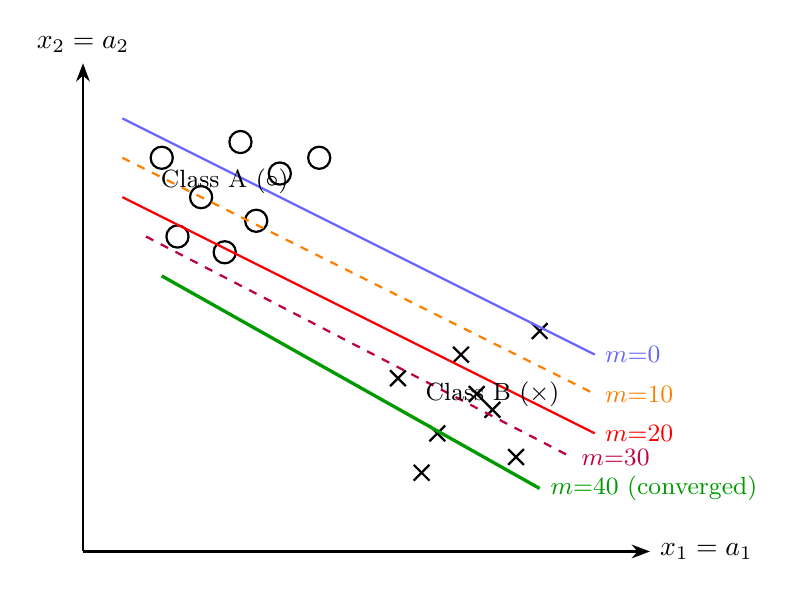
\begin{tikzpicture}[scale=1.0]
  %% Axes
  \draw[-{Stealth}, thick] (0,0) -- (7.2,0) node[right]{$x_1 = a_1$};
  \draw[-{Stealth}, thick] (0,0) -- (0,6.2) node[above]{$x_2 = a_2$};

  %% Class A points (circles) -- upper-left region
  \foreach \x/\y in {1.0/5.0, 1.5/4.5, 2.0/5.2, 1.2/4.0, 2.5/4.8,
                     1.8/3.8, 3.0/5.0, 2.2/4.2}{
    \draw[thick] (\x,\y) circle (4pt);
  }

  %% Class B points (crosses) -- lower-right region
  \foreach \x/\y in {4.5/1.5, 5.0/2.0, 5.5/1.2, 4.8/2.5, 5.2/1.8,
                     4.0/2.2, 5.8/2.8, 4.3/1.0}{
    \draw[thick] (\x-0.1,\y-0.1) -- (\x+0.1,\y+0.1);
    \draw[thick] (\x-0.1,\y+0.1) -- (\x+0.1,\y-0.1);
  }

  %% Decision boundaries at different epochs
  %% m=0
  \draw[blue!60, thick] (0.5,5.5) -- (6.5,2.5)
    node[right, font=\small]{$m{=}0$};
  %% m=10
  \draw[orange, thick, dashed] (0.5,5.0) -- (6.5,2.0)
    node[right, font=\small]{$m{=}10$};
  %% m=20
  \draw[red, thick] (0.5,4.5) -- (6.5,1.5)
    node[right, font=\small]{$m{=}20$};
  %% m=30
  \draw[purple, thick, dashed] (0.8,4.0) -- (6.2,1.2)
    node[right, font=\small]{$m{=}30$};
  %% m=40 (converged)
  \draw[green!60!black, very thick] (1.0,3.5) -- (5.8,0.8)
    node[right, font=\small, text=green!60!black]{$m{=}40$ (converged)};

  %% Class labels
  \node[font=\small] at (1.8,4.7) {Class A ($\circ$)};
  \node[font=\small] at (5.2,2.0) {Class B ($\times$)};

\end{tikzpicture}
\caption{Figure~4.3 (Yegnanarayana, 1999): Decision boundaries produced by
  the perceptron learning algorithm at epochs $m = 0, 10, 20, 30, 40$.
  The boundary wanders until convergence at $m = 40$.  Multiple valid
  boundaries exist; the one reached depends on initialisation.}
\label{fig:convergence}
\end{figure}

\subsection{Perceptron Learning Algorithm}
\label{subsec:algorithm}

\Cref{alg:perceptron} gives the complete training procedure.

\begin{algorithm}[ht]
\caption{Perceptron Learning Algorithm}
\label{alg:perceptron}
\SetAlgoLined
\DontPrintSemicolon
\KwIn{Training set $\{(\mathbf{x}^{(k)}, d^{(k)})\}_{k=1}^{N}$,
      learning rate $\eta > 0$, max epochs $T$}
\KwOut{Weight vector $\mathbf{w}$, bias $w_0$}

Initialise $\mathbf{w} \leftarrow \mathbf{0}$, $w_0 \leftarrow 0$\;
\For{epoch $t = 1$ \KwTo $T$}{
  $\text{errors} \leftarrow 0$\;
  \For{each sample $k = 1$ \KwTo $N$}{
    $z \leftarrow \sum_{i=0}^{n} w_i x_i^{(k)}$ \quad ($x_0^{(k)} \equiv 1$)\;
    $y^{(k)} \leftarrow f(z)$\;
    \If{$y^{(k)} \neq d^{(k)}$}{
      $w_i \leftarrow w_i + \eta\,(d^{(k)} - y^{(k)})\,x_i^{(k)}$
        \quad $\forall\, i$\;
      $\text{errors} \leftarrow \text{errors} + 1$\;
    }
  }
  \If{$\text{errors} = 0$}{
    \textbf{break} \quad (convergence reached)\;
  }
}
\end{algorithm}

\subsection{Multiclass Extension (Figure 4.9)}
\label{subsec:multiclass}

For $C > 2$ linearly separable classes one trains $C$ perceptrons in
parallel, one per class, using a one-versus-all strategy.  The $c$-th
perceptron is trained with samples from class $c$ as positive examples
and all remaining samples as negative examples.

\Cref{fig:multiclass} illustrates the network architecture (Fig.~4.9,
Yegnanarayana, 1999) and the corresponding decision regions for three
classes.

\begin{figure}[ht]
\centering
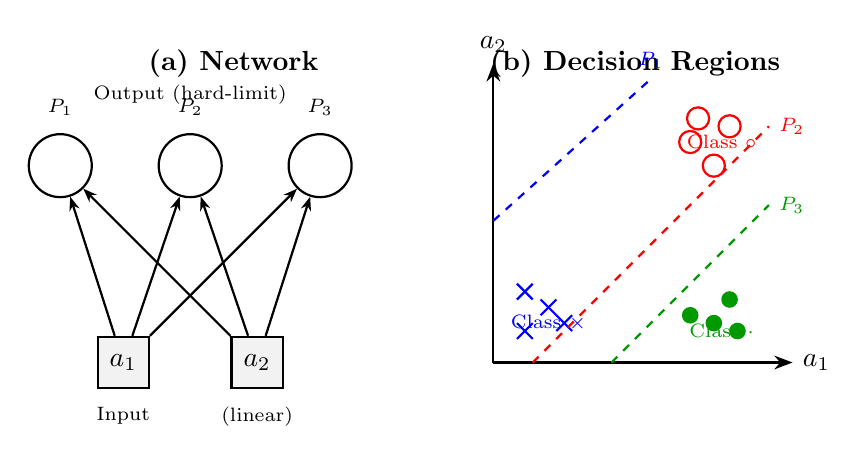
\begin{tikzpicture}[
    node distance=1.2cm and 1.8cm,
    unit/.style={circle, draw, minimum size=0.8cm, thick},
    inp/.style={rectangle, draw, minimum size=0.65cm, fill=gray!10, thick},
    arr/.style={-{Stealth[length=5pt]}, thick}
  ]

  %% ---- (a) Network architecture ----
  \node[font=\bfseries] at (2.2,3.8) {(a) Network};

  %% Input layer
  \node[inp] (a1) at (0.8, 0.0) {$a_1$};
  \node[inp] (a2) at (2.5, 0.0) {$a_2$};
  \node[font=\scriptsize, below=0.1cm of a1] {Input};
  \node[font=\scriptsize, below=0.1cm of a2] {(linear)};

  %% Output layer (3 perceptrons)
  \node[unit] (o1) at (0.0, 2.5) {};
  \node[unit] (o2) at (1.65,2.5) {};
  \node[unit] (o3) at (3.3, 2.5) {};
  \node[font=\scriptsize, above=0.1cm of o1] {$P_1$};
  \node[font=\scriptsize, above=0.1cm of o2] {$P_2$};
  \node[font=\scriptsize, above=0.1cm of o3] {$P_3$};
  \node[font=\scriptsize] at (1.65,3.4) {Output (hard-limit)};

  %% Connections (fully connected)
  \foreach \out in {o1, o2, o3}{
    \draw[arr] (a1) -- (\out);
    \draw[arr] (a2) -- (\out);
  }

  %% ---- (b) Decision regions ----
  \begin{scope}[xshift=5.5cm]
    \node[font=\bfseries] at (1.8,3.8) {(b) Decision Regions};

    \draw[-{Stealth}, thick] (0,0) -- (3.8,0) node[right]{$a_1$};
    \draw[-{Stealth}, thick] (0,0) -- (0,3.8) node[above]{$a_2$};

    %% Class X (crosses) -- lower-left
    \foreach \x/\y in {0.4/0.4, 0.7/0.7, 0.4/0.9, 0.9/0.5}{
      \draw[thick,blue] (\x-0.1,\y-0.1)--(\x+0.1,\y+0.1);
      \draw[thick,blue] (\x-0.1,\y+0.1)--(\x+0.1,\y-0.1);
    }

    %% Class O (circles) -- upper-right
    \foreach \x/\y in {2.5/2.8, 2.8/2.5, 3.0/3.0, 2.6/3.1}{
      \draw[thick,red] (\x,\y) circle (4pt);
    }

    %% Class dot (dots) -- lower-right
    \foreach \x/\y in {2.8/0.5, 3.0/0.8, 2.5/0.6, 3.1/0.4}{
      \fill[green!60!black] (\x,\y) circle (3pt);
    }

    %% Decision boundaries (slant lines)
    \draw[thick, blue,  dashed] (0.0,1.8) -- (2.0,3.6)
      node[above,font=\scriptsize]{$P_1$};
    \draw[thick, red,   dashed] (0.5,0.0) -- (3.5,3.0)
      node[right,font=\scriptsize]{$P_2$};
    \draw[thick, green!60!black, dashed] (1.5,0.0) -- (3.5,2.0)
      node[right,font=\scriptsize]{$P_3$};

    \node[font=\scriptsize,blue]         at (0.7,0.5) {Class $\times$};
    \node[font=\scriptsize,red]          at (2.9,2.8) {Class $\circ$};
    \node[font=\scriptsize,green!60!black] at (2.9,0.4) {Class $\cdot$};
  \end{scope}

\end{tikzpicture}
\caption{Figure~4.9 (Yegnanarayana, 1999): Multiclass perceptron.
  (a)~Network architecture: the input layer contains linear fan-out units;
  the output layer has one hard-limiting perceptron per class.
  (b)~Each perceptron learns a boundary separating its class from all others.}
\label{fig:multiclass}
\end{figure}

\begin{example}[title=Example -- Three-Class One-vs-All Training]
Suppose classes are $\times$, $\circ$, and $\bullet$.  Training proceeds
as follows:
\begin{enumerate}[noitemsep]
  \item Train $P_1$: set $\times$ samples as positive ($d=1$),
        $\circ$ and $\bullet$ as negative ($d=0$).
  \item Train $P_2$: set $\circ$ samples as positive, others as negative.
  \item Train $P_3$: set $\bullet$ samples as positive, others as negative.
\end{enumerate}
At inference, the class with the highest (or the only activated) output
wins.  The method extends to any number of classes, provided all are
linearly separable.
\end{example}

%% ══════════════════════════════════════════════════════════════════════
\section{Linearly Inseparable Problems}
\label{sec:inseparable}
%% ══════════════════════════════════════════════════════════════════════

\subsection{The XOR Problem}
\label{subsec:xor}

The XOR function is the canonical example of a linearly inseparable
problem.  The four data points $(0,0) \to 0$, $(0,1) \to 1$,
$(1,0) \to 1$, $(1,1) \to 0$ cannot be separated by any straight line in
the input plane.

\Cref{tab:xor-vs-or} compares the truth tables of OR and XOR, which have
identical inputs but differ in separability.

\begin{table}[ht]
\centering
\caption{OR (linearly separable) versus XOR (linearly inseparable).}
\label{tab:xor-vs-or}
\begin{tabular}{cc cc cc}
\toprule
\multicolumn{2}{c}{\textbf{Inputs}} & \multicolumn{2}{c}{\textbf{OR output}} & \multicolumn{2}{c}{\textbf{XOR output}} \\
\cmidrule(lr){1-2}\cmidrule(lr){3-4}\cmidrule(lr){5-6}
$x_1$ & $x_2$ & Value & Class & Value & Class \\
\midrule
0 & 0 & 0 & $-$ & 0 & $-$ \\
0 & 1 & 1 & $+$ & 1 & $+$ \\
1 & 0 & 1 & $+$ & 1 & $+$ \\
1 & 1 & 1 & $+$ & 0 & $-$ \\
\bottomrule
\end{tabular}

\vspace{4pt}
\small OR: three positives cluster in one region -- linearly separable.
XOR: positives at $(0,1)$ and $(1,0)$ form a diagonal pattern -- cannot
be enclosed by a single half-plane.
\end{table}

\begin{warningbox}[title=Warning -- Single Perceptron Cannot Solve XOR]
Running the perceptron learning algorithm on XOR data will cause the
decision boundary to wander indefinitely without convergence.  The
Convergence Theorem does not apply because no linearly separating
hyperplane exists.  Attempting to force convergence by capping iterations
will yield a sub-optimal boundary that always misclassifies at least one
sample.
\end{warningbox}

\subsection{Hard Problems and Representation Limits}
\label{subsec:hard-problems}

Problems that are not representable by a single-layer perceptron are
called \emph{hard problems} or \emph{representation problems} in the
neural network literature.  Formally:

\begin{definition}[Hard Problem]
\label{def:hard-problem}
A classification task is a \emph{hard problem} if no linear hyperplane
in the input space separates the classes, i.e., the data are
\emph{linearly inseparable}.
\end{definition}

Key properties of hard problems:
\begin{itemize}[noitemsep]
  \item The perceptron learning algorithm never converges -- the boundary
        oscillates without settling.
  \item The number of linearly separable Boolean functions
        \emph{decreases} as the input dimensionality $M$ increases.
  \item XOR and XNOR are the simplest hard problems for $M = 2$.
\end{itemize}

\subsection{Network Depth vs.\ Decision-Region Complexity (Figure 4.10)}
\label{subsec:depth-vs-region}

A landmark result from Lippmann (1987) -- reproduced in Yegnanarayana
(1999) as Figure~4.10 -- characterises exactly which decision regions
each network depth can realise.

\begin{table}[ht]
\centering
\caption{Decision-region complexity as a function of network depth
  (Lippmann, 1987; Yegnanarayana, 1999, Fig.~4.10).}
\label{tab:depth-regions}
\begin{tabular}{p{3.0cm} p{3.5cm} p{3.5cm} p{3.5cm}}
\toprule
\textbf{Network} & \textbf{Types of decision regions} &
\textbf{XOR problem} & \textbf{Classes with meshed regions} \\
\midrule
Two-layer\\(1 perceptron layer)
  & Half-plane bounded by a single hyperplane
  & Cannot solve (linearly inseparable)
  & Cannot handle \\
\midrule
Three-layer\\(1 hidden layer)
  & Convex open or closed region
  & Solves (convex hull around each class)
  & Cannot handle non-convex \\
\midrule
Four-layer\\(2 hidden layers)
  & Arbitrary region (limited only by neuron count)
  & Solves
  & Handles arbitrary shapes \\
\bottomrule
\end{tabular}
\end{table}

\begin{keyinsight}[title=Key Insight -- Depth Unlocks Richer Decision Regions]
Each additional perceptron layer qualitatively \emph{expands} the class
of representable decision regions.  A two-layer network creates linear
separations only.  A three-layer network combines linear boundaries into
\emph{convex} regions.  A four-layer network combines convex regions into
\emph{arbitrary} (potentially non-convex) shapes.  This hierarchical
composition of simple primitives is the geometric intuition behind the
power of deep networks.
\end{keyinsight}

%% ══════════════════════════════════════════════════════════════════════
\section{Multi-Layer Perceptron: Motivation and Definition}
\label{sec:mlp-motivation}
%% ══════════════════════════════════════════════════════════════════════

\subsection{From Single Layer to Multiple Layers}
\label{subsec:single-to-multi}

The inability of the single perceptron to handle linearly inseparable
data motivated a natural extension: inserting additional layers of
perceptrons \emph{before} the output layer.  Each perceptron in the new
hidden layer learns a linear hyperplane; the output layer then
\emph{combines} these hyperplanes into a more complex surface.

Formally, if the first perceptron layer produces outputs
$\mathbf{h} = (h_1, h_2, \ldots, h_p)$, the output layer operates on
$\mathbf{h}$ rather than the raw input $\mathbf{x}$:

\begin{align}
  \label{eq:mlp-forward}
  h_j &= f\!\left(\sum_{i=0}^{n} w_{ji}^{(1)} x_i\right),
    \quad j = 1, \ldots, p, \\[4pt]
  y_c &= f\!\left(\sum_{j=0}^{p} w_{cj}^{(2)} h_j\right),
    \quad c = 1, \ldots, C.
\end{align}

\subsection{Geometric Intuition}
\label{subsec:geometric-intuition}

Each hidden-layer perceptron creates a linear half-plane in the input
space.  The output perceptron performs a logical AND-like combination of
these half-planes, yielding a \emph{convex} region.  Two hidden layers
allow the second hidden layer to combine convex regions, producing
\emph{non-convex} or even disjoint regions.

As stated in the lecture:
\begin{quote}
\textit{``If I combine the outputs of two or more perceptrons in the next
perceptron layer, you get a modified hyper surface.  Convex surfaces will
be created.  The intersection of convex regions may produce any non-convex
region also.''}
\end{quote}

\begin{definition}[Convex Region]
\label{def:convex}
A region $\mathcal{R} \subseteq \mathbb{R}^n$ is \emph{convex} if for
every two points $\mathbf{p}, \mathbf{q} \in \mathcal{R}$, the line
segment $\lambda\mathbf{p} + (1-\lambda)\mathbf{q}$ for
$\lambda \in [0,1]$ lies entirely within $\mathcal{R}$.
\end{definition}

\subsection{MLP Architecture Diagram}
\label{subsec:mlp-diagram}

\Cref{fig:mlp} shows the four-layer feedforward network that can handle
arbitrary decision regions.

\begin{figure}[ht]
\centering
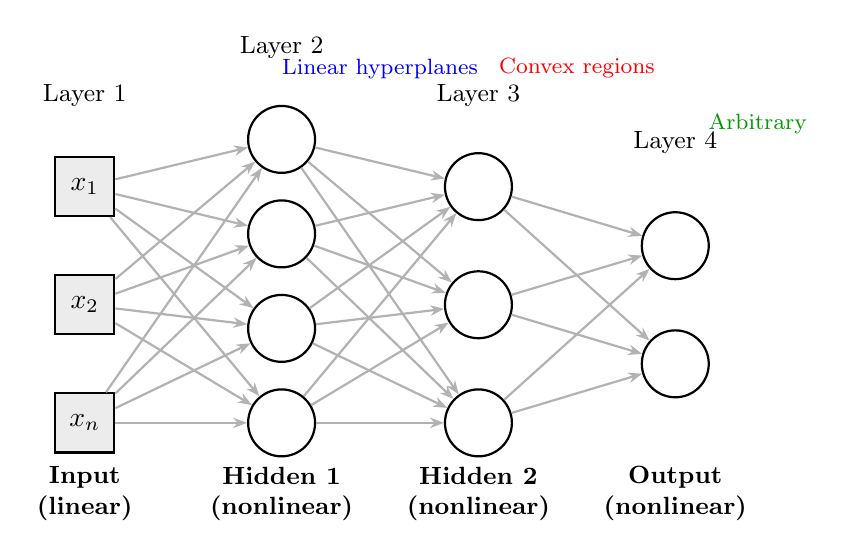
\begin{tikzpicture}[
    unit/.style={circle, draw, minimum size=0.85cm, thick, fill=white},
    inp/.style={rectangle, draw, minimum size=0.75cm, fill=gray!15, thick},
    arr/.style={-{Stealth[length=5pt]}, thick, gray!60},
    labl/.style={font=\small\bfseries, align=center}
  ]

  %% Layer positions (x-coords)
  \def\xI{0}
  \def\xH{2.5}
  \def\xHH{5.0}
  \def\xO{7.5}

  %% Input layer (3 units)
  \foreach \y/\name in {3.0/x1, 1.5/x2, 0.0/x3}{
    \node[inp] (\name) at (\xI, \y) {};
  }
  \node[inp] (x1l) at (\xI, 3.0) {$x_1$};
  \node[inp] (x2l) at (\xI, 1.5) {$x_2$};
  \node[inp] (x3l) at (\xI, 0.0) {$x_n$};
  \node[labl] at (\xI, -0.9) {Input\\(linear)};

  %% Hidden layer 1 (4 units)
  \foreach \y/\name in {3.6/h11, 2.4/h12, 1.2/h13, 0.0/h14}{
    \node[unit] (\name) at (\xH, \y) {};
  }
  \node[labl] at (\xH, -0.9) {Hidden 1\\(nonlinear)};

  %% Hidden layer 2 (3 units)
  \foreach \y/\name in {3.0/h21, 1.5/h22, 0.0/h23}{
    \node[unit] (\name) at (\xHH, \y) {};
  }
  \node[labl] at (\xHH, -0.9) {Hidden 2\\(nonlinear)};

  %% Output layer (2 units)
  \foreach \y/\name in {2.25/o1, 0.75/o2}{
    \node[unit] (\name) at (\xO, \y) {};
  }
  \node[labl] at (\xO, -0.9) {Output\\(nonlinear)};

  %% Connections Input -> H1
  \foreach \s in {x1l, x2l, x3l}{
    \foreach \t in {h11, h12, h13, h14}{
      \draw[arr] (\s) -- (\t);
    }
  }

  %% Connections H1 -> H2
  \foreach \s in {h11, h12, h13, h14}{
    \foreach \t in {h21, h22, h23}{
      \draw[arr] (\s) -- (\t);
    }
  }

  %% Connections H2 -> Output
  \foreach \s in {h21, h22, h23}{
    \foreach \t in {o1, o2}{
      \draw[arr] (\s) -- (\t);
    }
  }

  %% Layer labels
  \node[font=\small, above=0.3cm] at (\xI,  3.6) {Layer 1};
  \node[font=\small, above=0.3cm] at (\xH,  4.2) {Layer 2};
  \node[font=\small, above=0.3cm] at (\xHH, 3.6) {Layer 3};
  \node[font=\small, above=0.3cm] at (\xO,  3.0) {Layer 4};

  %% Brace annotations
  \node[font=\footnotesize, blue, align=center] at (3.75, 4.5)
    {Linear hyperplanes};
  \node[font=\footnotesize, red,  align=center] at (6.25, 4.5)
    {Convex regions};
  \node[font=\footnotesize, green!60!black, align=center, right] at (7.8, 3.8)
    {Arbitrary};

\end{tikzpicture}
\caption{Four-layer feedforward network (Multi-Layer Perceptron).
  Layer 1 (input) distributes data; Layer 2 (first hidden) creates linear
  hyperplanes; Layer 3 (second hidden) combines them into convex regions;
  Layer 4 (output) further combines these into arbitrary decision regions.}
\label{fig:mlp}
\end{figure}

\begin{definition}[Multi-Layer Perceptron (MLP)]
\label{def:mlp}
A \emph{Multi-Layer Perceptron} is a fully connected feedforward neural
network consisting of:
\begin{itemize}[noitemsep]
  \item An \emph{input layer} of linear fan-out units (not counted as a
        perceptron layer);
  \item One or more \emph{hidden layers} of nonlinear perceptrons;
  \item An \emph{output layer} of nonlinear perceptrons.
\end{itemize}
A network with three or more total layers (i.e., two or more perceptron
layers) is called a multi-layer perceptron.
\end{definition}

\subsection{Relationship Between Layers and Region Complexity}
\label{subsec:layers-regions}

\begin{theorem}[Layer-Region Correspondence]
\label{thm:layers-regions}
For a feedforward network with hard-limiting (step function) units:
\begin{itemize}[noitemsep]
  \item \textbf{1 perceptron layer} (2-layer network): produces linear
        hyperplane boundaries -- half-plane regions only.
  \item \textbf{2 perceptron layers} (3-layer network): produces
        convex regions formed by the intersection of linear hyperplanes.
  \item \textbf{3 perceptron layers} (4-layer network): produces
        arbitrary regions formed by the union of convex regions.
\end{itemize}
\end{theorem}

The theorem also holds when the step function is replaced by a continuous
nonlinear activation (e.g., sigmoid), as noted by the instructors:
``Similar behavior is expected from a multi-layer feed-forward network
when the output functions of the units are continuous non-linear
functions, such as sigmoid.''

\subsection{Number of Units and Surface Complexity}
\label{subsec:unit-count}

Key design parameters govern the expressiveness of the network:

\begin{itemize}[noitemsep]
  \item The number of units in the \textbf{first hidden layer} determines
        the \emph{shape} of the dividing surfaces (how many hyperplane
        ``facets'' can be combined).
  \item The number of units in the \textbf{output layer} determines the
        \emph{number of classes} the network can discriminate.
  \item Adding more units to the hidden layers increases the complexity
        of achievable decision boundaries.
\end{itemize}

%% ══════════════════════════════════════════════════════════════════════
\section{The Problem with the Perceptron}
\label{sec:problem}
%% ══════════════════════════════════════════════════════════════════════

\subsection{Non-Uniqueness of the Separating Hyperplane (V06)}
\label{subsec:non-unique}

Even when the data \emph{are} linearly separable, the perceptron has a
fundamental limitation: it finds \emph{some} separating hyperplane, but
has \emph{no mechanism} to select the \emph{best} one.

As illustrated in the lecture (timestamp 01:05:00), infinitely many valid
hyperplanes A, B, C, D can all separate the two classes, yet the
perceptron stops at whichever it encounters first.

\begin{align}
  \label{eq:loss-hinge}
  \mathcal{L}_{\text{hinge}}(\mathbf{w}) =
  \sum_{k=1}^{N} \max\!\bigl(0,\; -\,y^{(k)}\,\mathbf{w}^{\top}\mathbf{x}^{(k)}\bigr),
\end{align}

where $y^{(k)} \in \{-1, +1\}$.  The perceptron loss is zero for any
correctly separating hyperplane regardless of the margin -- it cannot
distinguish between a boundary that passes close to the data and one that
has a wide margin.

\subsection{Contrast with Support Vector Machines}
\label{subsec:svm-comparison}

A student question during the lecture highlighted an important contrast:

\begin{quote}
\textit{Student: ``In SVM we select a hyperplane that maximises the
margin.  Does the perceptron also maximise the margin?''}

\textit{Instructor: ``Here it is not a maximum margin classifier.
That is where I told you, there are infinite solutions possible.  For a
maximum margin classifier, the line should come exactly in the centre so
that all the samples are equally distanced from positive and negative
examples.  In the neural network, there is no maximum margin classifier.''}
\end{quote}

\Cref{tab:perceptron-svm} contrasts the two approaches.

\begin{table}[ht]
\centering
\caption{Perceptron vs.\ Support Vector Machine (SVM).}
\label{tab:perceptron-svm}
\begin{tabular}{lll}
\toprule
\textbf{Property} & \textbf{Perceptron} & \textbf{SVM} \\
\midrule
Objective          & Correct classification & Maximum margin \\
Solution uniqueness & Any valid boundary     & Unique (maximum-margin) \\
Optimality         & No guarantee           & Optimal (max margin) \\
Convergence        & Finite if separable    & Always (via QP) \\
Non-linear case    & Needs MLP / more layers & Kernel trick \\
Update rule        & Perceptron rule        & Quadratic programming \\
\bottomrule
\end{tabular}
\end{table}

\begin{keyinsight}[title=Key Insight -- Perceptron Finds a Solution but Not the Best]
The perceptron's lack of a margin optimisation criterion is one of its
principal weaknesses.  This limitation motivated two parallel lines of
research: (1) the Support Vector Machine, which explicitly maximises the
margin, and (2) gradient-based training of multi-layer networks with
differentiable loss functions, which can be designed to prefer
well-generalising solutions.
\end{keyinsight}

%% ══════════════════════════════════════════════════════════════════════
\section{Activation Functions}
\label{sec:activations}
%% ══════════════════════════════════════════════════════════════════════

\subsection{Overview}
\label{subsec:activations-overview}

The activation function $f$ transforms the weighted sum $z =
\sum_i w_i x_i + b$ into the neuron's output.  Although the classical
perceptron uses the step function, the lecture introduces several
alternatives that make the model more flexible and differentiable.

\subsection{Step Function}
\label{subsec:step}

\begin{equation}
  \label{eq:step-fn}
  f_{\text{step}}(z) =
  \begin{cases}
    1 & z \geq 0, \\
    0 & z < 0.
  \end{cases}
\end{equation}

Output: $\{0, 1\}$.  Non-differentiable at the origin; used in the
classical perceptron.

\subsection{Sigmoid Function}
\label{subsec:sigmoid}

\begin{equation}
  \label{eq:sigmoid}
  f_{\sigma}(z) = \frac{1}{1 + e^{-z}}.
\end{equation}

Output: $(0, 1)$ -- interpretable as a probability.  Differentiable
everywhere; the ``S-shaped'' curve is bounded and monotone.  Preferred
when probabilistic outputs are required.

\subsection{Hyperbolic Tangent}
\label{subsec:tanh}

\begin{equation}
  \label{eq:tanh}
  f_{\tanh}(z) = \tanh(z) = \frac{e^{z} - e^{-z}}{e^{z} + e^{-z}}.
\end{equation}

Output: $(-1, +1)$.  Zero-centred, which can speed up training.
Commonly used in recurrent neural networks (LSTMs, GRUs) for hidden-state
activations.

\subsection{Rectified Linear Unit (ReLU)}
\label{subsec:relu}

\begin{equation}
  \label{eq:relu}
  f_{\text{ReLU}}(z) = \max(0, z).
\end{equation}

Output: $[0, \infty)$.  Computationally efficient; avoids vanishing
gradients for positive inputs.  Widely used in convolutional neural
networks (CNNs).

\begin{table}[ht]
\centering
\caption{Comparison of common activation functions.}
\label{tab:activations}
\begin{tabular}{lcccc}
\toprule
\textbf{Function} & \textbf{Formula} & \textbf{Range} &
\textbf{Differentiable} & \textbf{Typical use} \\
\midrule
Step     & $\mathbf{1}[z \geq 0]$             & $\{0,1\}$   & No (at 0) & Classical perceptron \\
Sigmoid  & $1/(1+e^{-z})$                      & $(0,1)$     & Yes       & Binary classification \\
Tanh     & $(e^z - e^{-z})/(e^z + e^{-z})$    & $(-1,1)$    & Yes       & RNNs, LSTMs \\
ReLU     & $\max(0, z)$                        & $[0,\infty)$& No (at 0) & CNNs, deep networks \\
\bottomrule
\end{tabular}
\end{table}

\begin{example}[title=Example -- Sigmoid vs.\ Step on the Same Input]
Consider $z = 0.12$ (from the bias example in \cref{sec:bias}).
\begin{align*}
  f_{\text{step}}(0.12)   &= 1, \\
  f_{\sigma}(0.12)         &= \frac{1}{1 + e^{-0.12}} \approx 0.530, \\
  f_{\tanh}(0.12)          &= \tanh(0.12) \approx 0.119, \\
  f_{\text{ReLU}}(0.12)   &= 0.12.
\end{align*}
The step function gives a hard binary decision.  The sigmoid provides a
probability near 0.53, reflecting mild confidence.  Tanh gives a
zero-centred near-zero output.  ReLU passes the value through unchanged
(since it is positive).
\end{example}

%% ══════════════════════════════════════════════════════════════════════
\section{Summary and Conclusion}
\label{sec:conclusion}
%% ══════════════════════════════════════════════════════════════════════

\subsection{Session Summary}
\label{subsec:summary}

Session~04 completed the perceptron coverage and laid the conceptual
groundwork for Multi-Layer Perceptrons.  The key results are:

\begin{enumerate}[label=\textbf{\arabic*.}, noitemsep]
  \item \textbf{Bias is a learned parameter.}  It shifts the decision
        boundary away from the origin, enabling classification of patterns
        that pure weighted sums cannot handle.

  \item \textbf{The Perceptron Convergence Theorem.}  For linearly
        separable data, the perceptron learning algorithm converges in a
        finite number of steps to a valid separating hyperplane.

  \item \textbf{XOR and XNOR are not linearly separable.}  Of the 16
        two-input Boolean functions, only these two cannot be learned by a
        single perceptron.  The number of linearly separable functions
        decreases as dimensionality increases.

  \item \textbf{The perceptron finds a boundary but not the best one.}
        There are infinitely many valid separating hyperplanes; the
        perceptron has no margin-optimisation mechanism.

  \item \textbf{Depth enables richer decision regions.}  Two-layer
        networks create half-planes; three-layer networks create convex
        regions; four-layer networks create arbitrary regions
        (Lippmann, 1987).

  \item \textbf{MLP as the solution to hard problems.}  Multi-Layer
        Perceptrons with two or more hidden perceptron layers can
        represent any decision region and are not limited to linearly
        separable tasks.

  \item \textbf{Activation function flexibility.}  By replacing the step
        function with sigmoid, tanh, or ReLU, the same network
        architecture can be used for probability estimation, zero-centred
        regression, or sparse activation respectively.
\end{enumerate}

\subsection{Looking Ahead}
\label{subsec:ahead}

The conceptual framework established here -- that depth unlocks
expressiveness -- is the foundation of all modern deep learning.  The
next challenge, addressed in subsequent sessions, is \emph{how to train}
a multi-layer network.  The perceptron learning rule does not extend
directly to hidden layers (there is no desired output to compare against
for intermediate nodes).  The solution is \textbf{backpropagation} with
gradient-based optimisation, which uses the chain rule to propagate error
signals from the output back through all hidden layers.

\begin{keyinsight}[title=Key Insight -- The Road from Perceptron to Deep Learning]
The perceptron story -- simple model, guaranteed convergence for easy
problems, fundamental limitation for hard problems -- is a microcosm of
the entire history of machine learning.  Every advance in deep learning
(MLPs, CNNs, RNNs, Transformers) can be read as a response to a specific
limitation of simpler models.  Understanding why a perceptron \emph{fails}
on XOR is therefore not just a historical curiosity: it is the seed from
which the entire field grew.
\end{keyinsight}

%% ══════════════════════════════════════════════════════════════════════
%%  REFERENCES
%% ══════════════════════════════════════════════════════════════════════
\newpage
\begin{thebibliography}{9}

\bibitem{yegna1999}
B.~Yegnanarayana,
\textit{Artificial Neural Networks},
PHI Learning, New Delhi, 1999.

\bibitem{lippmann1987}
R.~P.~Lippmann,
``An introduction to computing with neural nets,''
\textit{IEEE ASSP Magazine}, vol.~4, no.~2, pp.~4--22, Apr.~1987.

\bibitem{rosenblatt1958}
F.~Rosenblatt,
``The perceptron: A probabilistic model for information storage and
organization in the brain,''
\textit{Psychological Review}, vol.~65, no.~6, pp.~386--408, 1958.

\bibitem{minsky1969}
M.~Minsky and S.~Papert,
\textit{Perceptrons: An Introduction to Computational Geometry},
MIT Press, Cambridge, MA, 1969.

\bibitem{rumelhart1986}
D.~E.~Rumelhart, G.~E.~Hinton, and R.~J.~Williams,
``Learning representations by back-propagating errors,''
\textit{Nature}, vol.~323, pp.~533--536, 1986.

\end{thebibliography}

\clearpage

\end{document}
